% don't remove the folling lines, and edit the defintion of \main if needed
\documentclass[../report.tex]{subfiles}
\providecommand{\main}{..}
\IfEq{\jobname}{\currfilebase}{\AtEndDocument{\biblio}}{}
\IfEq{\jobname}{\currfilebase}{%file for shortcuts

\newcommand{\nch}{\ensuremath{N_{\mathrm {ch}}\xspace}}
\newcommand{\Ncoll}{\ensuremath{N_{\mathrm {coll}}}}
\newcommand{\Npart}{\ensuremath{N_{\mathrm {part}}}}
\newcommand{\dNdeta}{\mathrm{d}N_\mathrm{ch}/\mathrm{d}\eta}
\newcommand{\snn}         {\ensuremath{\sqrt{s_{\mathrm {NN}}}}}
\newcommand{\kT}          {\ensuremath{k_{\mathrm {T}}}}

\newcommand{\pp}          {pp}
\newcommand{\pPb}         {pPb}
\newcommand{\pA}          {pA}
\newcommand{\PbPb}        {PbPb}
\newcommand{\AuAu}        {AuAu}
\newcommand{\CuCu}        {CuCu}
\newcommand{\pAu}         {pAu}
\newcommand{\dAu}         {dAu}
\newcommand{\lsim}        {\,{\buildrel < \over {_\sim}}\,}
\newcommand{\gsim}        {\,{\buildrel > \over {_\sim}}\,}
\newcommand{\co}[1]       {\relax}
\newcommand{\nl}          {\newline}
\newcommand{\el}          {\\\hline\\[-0.4cm]}}{}
% until here

\begin{document}

\section{Electromagnetic radiation}
\label{chapter:electromagnetic_radiation}

\textbf{Coordinators}: Michael Weber (Stefan Meyer Institute Vienna, Austrian Academy of Sciences) 
\linebreak
\textbf{Contributors}: 
		Raphaelle Bailhache (Goethe-University Frankfurt), 
        Rupa Chatterjee (VECC Calcutta),
		Torsten Dahms (Excellence Cluster Universe, Technical University Munich), 
		Taku Gunji (Center for Nuclear Study, Graduate School of Science, the University of Tokyo), 
        Min He (Nanjing University of Science and Technology),
        Spencer Klein (Lawrence Berkeley National Laboratory), 
        Ana Marin (GSI Darmstadt), 
        Dmitri Peresunko (National Research Centre Kurchatov Institute, Moscow),  
        Ralf Rapp (Texas A\&M University), 
        Klaus Reygers (Heidelberg University), 
        Taesoo Song (University of Gie{\ss}en), 
        Antonio Uras (Universit{\'e} de Lyon, CNRS/IN2P3, IPN-Lyon),
        Gojko Vujanovic (Ohio State University and Wayne State University)

%The general guideline to include people who have contributed to either text, plots or substantially to important discussions. If you have doubt, please contact the conveners.

%Acknowledgements: 
%Please add any needed acknowledgements (funding agencies etc.) 
The strongly interacting system formed in ultrarelativistic heavy-ion collisions 
%is considered to be in thermal equilibrium and therefore
emits electromagnetic radiation that can be detected using different probes: real {\it direct} photons %with low momentum
or virtual photons measurable via dilepton pairs. 
Direct photons can be split into {\it prompt} photons, emitted by the partons of colliding nuclei during their inter-penetration, and {\it thermal} photons, emitted by the almost thermalized hot system. 
For dileptons these contributions are called Drell-Yan and thermal, respectively.
In contrast to real photons, dileptons carry a mass and thus can be used to study the decay of massive particles, such as the in-medium modified spectral shape of vector mesons, the \PGr meson being the most prominent one, and the search for particles beyond the Standard Model, \eg dark photons. In this section, we outline the measurement of photons via calorimetry and the so-called photon conversion method, as well as dielectron (\Pepem), and dimuon (\PGmpGmm) pairs in AA collisions in the ALICE detector at the LHC. Moreover, the photoproduction of dilepton pairs in peripheral collisions and the expected sensitivity for the search of dark photons is discussed in subsections \ref{sec:dileptons:peripheral} and \ref{sec:dileptons:darkphotons}, respectively. We begin with a short review of previous experimental results together with a summary of the basic theoretical models employed to describe these data.


\subsection{Thermal radiation}
\label{sec:thermalradiation}
%Contributed by Michael Weber, Torsten Dahms

Electromagnetic radiation from the hot and dense system formed in ultrarelativistic heavy-ion collisions was measured for the first time at the SPS in the form of real photons by WA98~\cite{Aggarwal:2000th}. The direct photon spectrum measured in \PbPb{} collisions at $\sqrtsNN = \unit[17.3]{\UGeV}$ showed an excess above the extrapolated prompt photon signal based on measurements in proton induced reactions. 
The excess is described by large variety of hydrodynamic and cascade models (see \cite{Peitzmann:2001mz} for review), most of them assume creation of QGP phase.
%The excess is successfully described by a fireball model that includes a 30\% contribution from a quark--gluon plasma (QGP) phase~\cite{Turbide:2003si}. 
Also at the SPS, a modification of low-mass dilepton pairs in S--Au and Pb--Au collisions relative to the expectation of in-vacuum hadron decays was observed by CERES~\cite{Agakishiev:1995xb,Agakishiev:1997au,Adamova:2002kf,Agakichiev:2005ai,Adamova:2006nu} and studied with high precision by NA60 in In--In collisions~\cite{Arnaldi:2006jq,Arnaldi:2007ru,Arnaldi:2008fw,Specht:2010xu}. The data are consistent with a modified \PGr spectral function that is melting and degenerating with $\PQq\PAQq$ radiation via the coupling to baryons in the dense medium, in which chiral symmetry is at least partially restored~\cite{Rapp:1995zy,Rapp:1999us,Rapp:2009yu,Bazavov:2011nk,Hohler:2013eba}. On the other hand, the data cannot be described with a dropping mass scenario, in which the \PGr mass drops to zero as chiral symmetry is restored~\cite{Brown:1991kk}. Beyond the issue of chiral symmetry restoration, NA60 measured an excess of prompt dimuons in the intermediate mass region between the \PGf and the \PJGy masses~\cite{Arnaldi:2007ru,Arnaldi:2008fw}. Contrary to transverse-mass spectra of the dimuon continuum at lower masses, this excess shows no increase of the exponential inverse slope with mass, \ie blue shift, that is typical for radial flow. This suggests that the source of this enhancement is from the earliest phase of the collision, before significant radial flow has built up. 
This supports the idea that the inverse slope of the invariant mass spectrum is insensitive to the expansion of the medium and therefore a true measure of the average temperature. NA60 measured a value of $T=\unit[205\pm12]{\UMeV}$~\cite{Specht:2010xu}, which significantly exceeds the temperature of $\unit[154\pm9]{\UMeV}$, above which the formation of a Quark--Gluon Plasma (QGP) has been predicted~\cite{Borsanyi:2010bp,Bazavov:2014pvz}.

At RHIC energies, PHENIX and STAR have measured an enhancement of \Pepem pairs in the low mass region in Au--Au collisions~\cite{Adare:2009qk,Adare:2015ila,Adamczyk:2013caa,Adamczyk:2015mmx} that can be described with the same model of collisional broadening as used at the SPS. STAR measured that the enhancement above the hadron decay background does not change with collision energy between $\sqrtsNN=\unit[19]{}$ and \unit[200]{\UGeV}~\cite{Adamczyk:2015mmx}. Despite a marked decrease of the net-baryon chemical potential in this energy range, the total baryon plus anti-baryon density does not change much, providing further evidence that the $\PGr$ coupling to baryons and antibaryons is responsible for the enhancement.
Real direct photon production in Au--Au collisions was measured by PHENIX~\cite{Adare:2008ab,Adare:2014fwh,Adare:2018wgc}. An excess was observed compared to binary scaled direct photon production in \pp{} collisions. The signal was measured via quasi-real virtual photons as well as real photons converting in detector material. The excess yield at low \pT{} appears to have a universal multiplicity dependence, scaling with the charged-particle multiplicity at midrapidity to the power of about 1.25, independent of collision energy between $\sqrtsNN = \unit[39]{}$ and \unit[200]{\UGeV}~\cite{Adare:2018wgc}. The transverse momentum spectrum of the excess yield has an exponential inverse slope of $T=\unit[221\pm19\pm19]{\UMeV}$ for central collisions and values close to that for other centralities. The spectrum, however, is strongly blue shifted by radial flow in the later stages of the fireball radiation, which is further supported by a sizeable elliptic flow ($v_2$) of the direct photon signal~\cite{Adare:2011zr}. Therefore, the inverse slope cannot directly be interpreted as an average temperature, which highlights the importance of thermal dilepton measurements as a function of invariant mass. The direct photon $v_2$ is indeed comparable to the $v_2$ of pions, which suggests late emission of direct photons dominated by the hadronic phase \cite{vanHees:2011vb}. To simultaneously describe the elliptic flow effect, as well as the large direct photon excess, which implies early production, poses a significant challenge to theoretical models.

First results of direct photon production at the LHC also show an indication of an excess production due to thermal radiation~\cite{Adam:2015lda}. The elliptic flow measurement~\cite{Acharya:2018bdy}, however, does not cause the same challenges to models, since the experimental uncertainties are still large at this point.
The reduction of systematic uncertainties of the direct photon measurement is the main objective for Run 3 to improve its significance. Moreover, a low magnetic field run will allow one to access the $\pT < \unit[1]{\UGeVc}$ region where the thermal photon production increases rapidly. Theoretical calculations of thermal and prompt photon productions are available at $\sqrtsNN = \unit[5.02]{\UTeV}$ (Fig.~\ref{fig:LHCExpectations_RealPhotons}) \cite{Paquet:2015lta,Paquet:2016ime,Paquet:2017wji,Dasgupta:2018pjm,vanHees:2014ida}. An increase by a factor $\sim$ 1.5 at about $\pT \approx \unit[1]{\UGeVc}$ and by a factor 1.5 to 2 for the prompt photons is predicted compared to yields at $\sqrtsNN = \unit[2.76]{\UTeV}$. The predicted thermal photon elliptic flow parameters for central collisions are close to each other at the two LHC energies  and are very small. Differences become larger as one goes towards peripheral collisions. Simultaneous measurements of photon yields and photon flow with high accuracy and lower \pT{} reach will provide constraints to theoretical models.
%-----------------------------------------------------------------------%
\begin{figure}[htb]
\centering
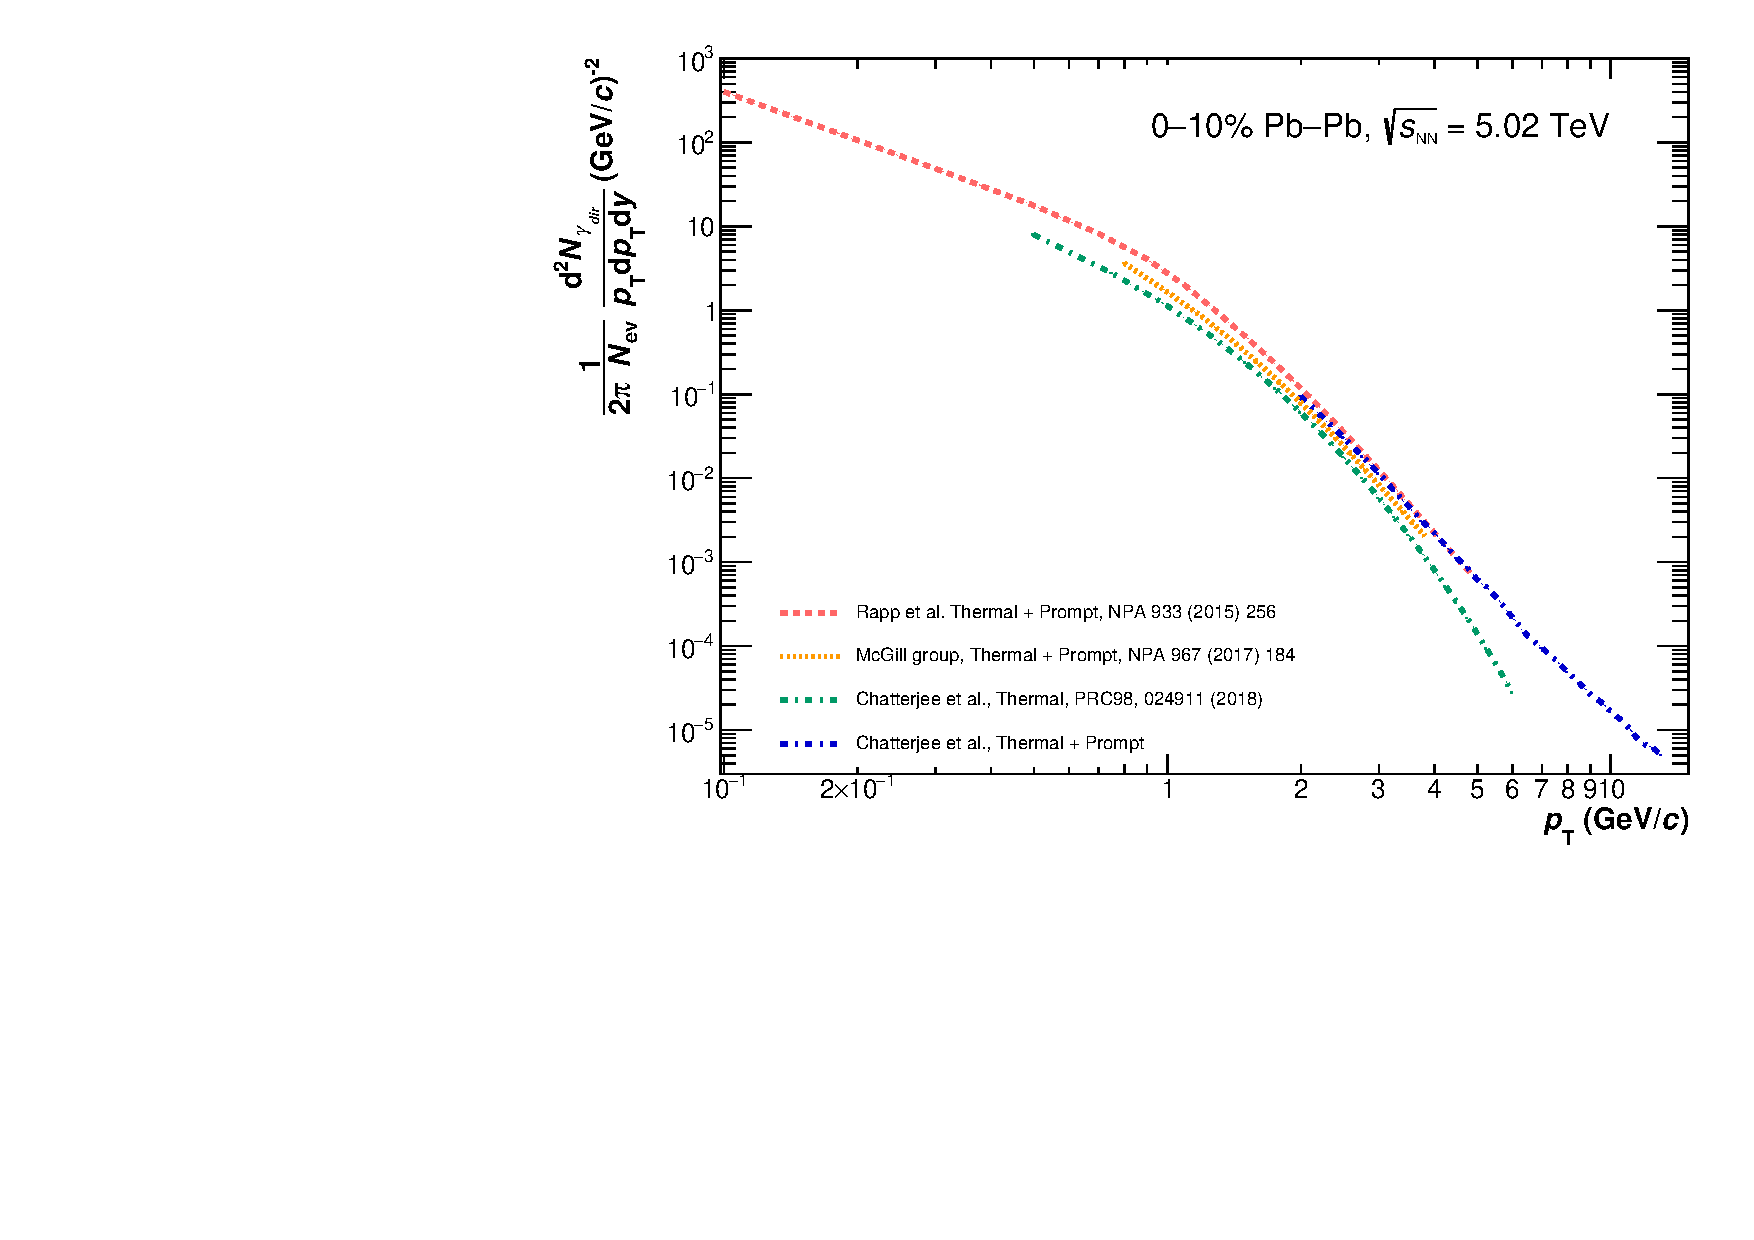
\includegraphics[width=0.6\textwidth]{\main/thermalradiation/figs/DirectPhotonYields5TeVYR.pdf}
\caption{Direct photon differential invariant yield for central 0--10\% \PbPb{} collisions at $\sqrtsNN = \unit[5.02]{\UTeV}$ as predicted by several models \cite{Paquet:2015lta,Paquet:2016ime,Paquet:2017wji,Dasgupta:2018pjm,vanHees:2014ida}.}
\label{fig:LHCExpectations_RealPhotons}
\end{figure}
%-----------------------------------------------------------------------%


Dilepton measurements by ALICE at the LHC are not yet sensitive to possible low-mass enhancement and thermal signals~\cite{Acharya:2018nxm}. A precise measurement of the low-mass dielectron continuum will be one of the main objectives of the ALICE physics programme during the LHC Run 3 and 4. In the meanwhile, the dominant background of dielectrons from correlated semileptonic open heavy-flavour decays is utilised to learn more about open heavy-flavour production in \pp{} collisions at LHC energies~\cite{Acharya:2018ohw,Acharya:2018kkj}.


%-----------------------------------------------------------------------%
\begin{figure}[htb]
\centering
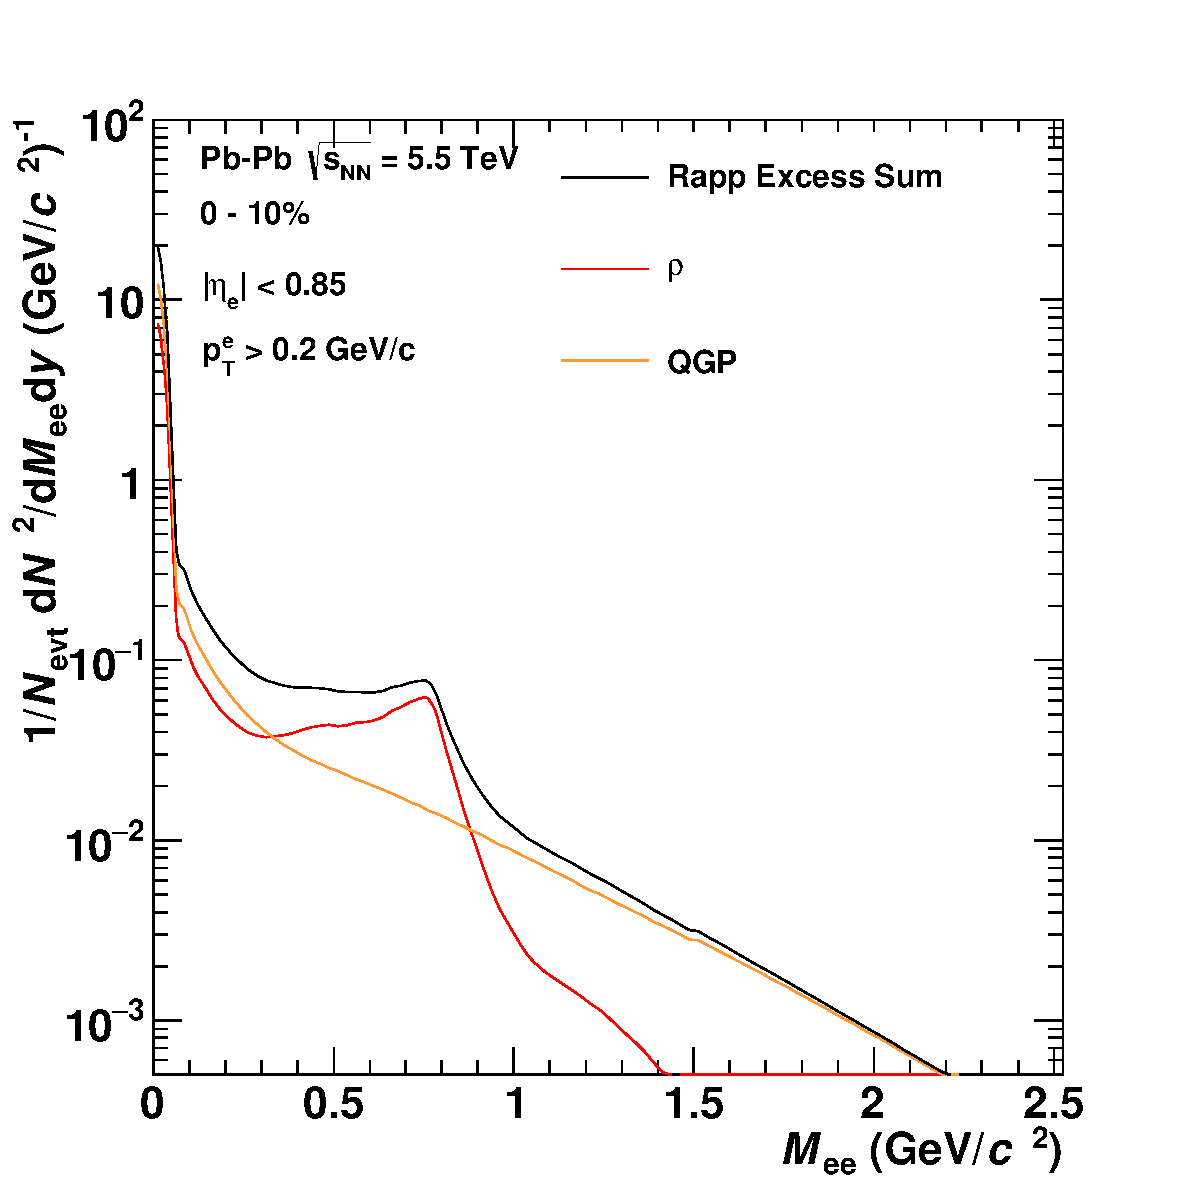
\includegraphics[width=0.45\textwidth]{\main/thermalradiation/figs/finalPlotsLowB_YR_Rapp_Excess_ITSCyl0_IPcut1_events2500000000000}
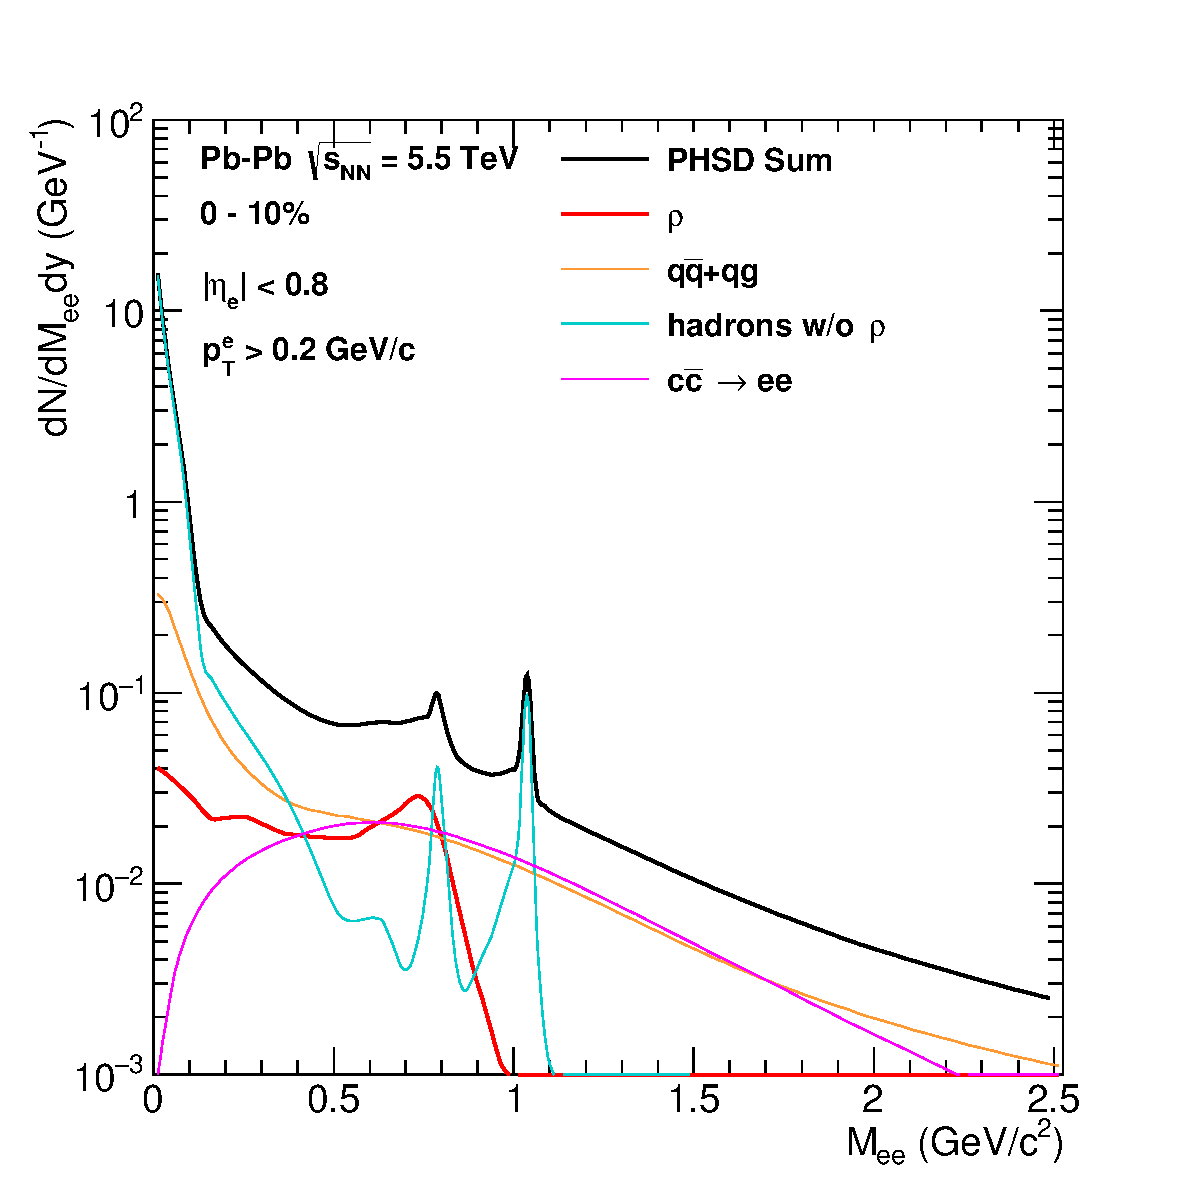
\includegraphics[width=0.45\textwidth]{\main/thermalradiation/figs/finalPlotsLowB_YR_PHSD_signalsOnly_ITSCyl0_IPcut1_events2500000000000}
\caption{Model predictions for the invariant mass spectrum of \Pepem pairs in central (0--10\%) \PbPb{} collisions at $\sqrtsNN = \unit[5.5]{\UTeV}$. Left panel: in-medium radiation plus decays of the \PGr meson at the end of the system evolution. Right panel: Expectations from the PHSD model including the in-medium \PGr meson, $\PQq\PAQq\rightarrow\Pepem$, $\PQq\PAQq\rightarrow\Pepem\Pg$, and $\PQq(\PAQq)\Pg\rightarrow\Pepem\PQq(\PAQq)$, hadronic sources, and semileptonic decays of $c\bar{c}$ and $b\bar{b}$.}
\label{fig:LHCExpectations_Rapp_pHSD}
\end{figure}
%-----------------------------------------------------------------------%

An approach that has been proven to provide a quantitative description of the existing dilepton results \cite{Rapp:2011is} is based on two ingredients that are put into a realistic space-time evolution \cite{Rapp:2000pe}. The thermal dilepton radiation is modelled by emission rates from the hadronic phase and the Quark--Gluon Plasma \cite{vanHees:2007th,Rapp:2009yu}. A hadronic many-body approach \cite{Rapp:1999us} is used for the medium-modified spectral functions of $\PGr$ and $\PGo$ mesons. In addition, the equation of state is updated to a cross-over transition around $T_{\rm c}=\unit[170]{\UMeV}$ extracted from with recent lattice QCD computations, and hadro-chemical freezeout at $T_{\rm chem}=\unit[160]{\UMeV}$ \cite{He:2011zx}. Figure \ref{fig:LHCExpectations_Rapp_pHSD} (left) shows the calculations performed for central \PbPb{} collisions at $\sqrtsNN = \unit[5.5]{\UTeV}$ for in-medium radiation plus decays of the \PGr meson at the end of the system evolution. The pair-yield is estimated for the rapidity range $|y_{\rm e}|<0.85$ and transverse momentum of single electrons $\pT^{\rm e}>\unit[0.2]{\UGeVc}$ and is normalized to the number of events $N_{\rm evt}$. 
 
A complementary approach to study dilepton spectra and thermal radiation is provided by the parton-hadron-string dynamics (PHSD) transport approach, which also successfully describes the existing experimental data \cite{Linnyk:2015rco,Cassing:2009vt}. The in-medium modification of the \PGr meson is incorporated in PHSD by an off-shell transport of vector mesons with a dynamically changing set of spectral functions \cite{Bratkovskaya:2007jk} evolving towards the vacuum spectral function at the end of the collision history. The electromagnetic radiation of the QGP is modelled by $\PQq\PAQq\rightarrow\Pepem$, $\PQq\PAQq\rightarrow\Pepem\Pg$, and $\PQq(\PAQq)\Pg\rightarrow\Pepem\PQq(\PAQq)$ using effective propagators for quarks and gluons from a dynamical quasi-particle model \cite{Linnyk:2010vb}. Figure \ref{fig:LHCExpectations_Rapp_pHSD} (right) shows both contributions to the dielectron spectrum in central \PbPb{} collisions at $\sqrtsNN = \unit[5.5]{\UTeV}$ calculated from PHSD together with other sources of dielectrons: decays of long-lived light mesons into \Pepem or X\Pepem (the so-called hadronic cocktail) and the semileptonic decay of hadrons containing heavy quarks, such as \PD and \PB mesons. 

Important input for models aiming to describe the dilepton yield at LHC energies are the in-medium spectral functions for the vector mesons, most importantly the \PGr meson, as well as the photon and dilepton rates from the QGP. For the latter, Lattice QCD calculations, which are currently limited to the quenched approximation, will hopefully be extended (\eg larger lattices, especially in the time direction, or facilitating extrapolations to the continuum limit) and be available in higher accuracy for realistic systems including light dynamical degrees of freedom in the future. Recent updates on calculations of the photon rate \cite{Ghiglieri:2016tvj}, the electrical conductivity \cite{Aarts:2014nba}, and dilepton rates \cite{Ding:2016hua} are promising.
The photons and dilepton rates from Lattice calculations should in the future be combined with dynamical models like those in Fig.~\ref{fig:LHCExpectations_Rapp_pHSD}, thus improving their results. In addition, the in-medium spectral functions could also use direct input from Lattice QCD \cite{Aarts:2005hg,Brandt:2015aqk} or from a functional renormalization group approach \cite{Jung:2016yxl}. These models can further be refined by including the effects of dissipation, and in that case the electrical conductivity will become of interest to both the dynamical evolution of the medium as well as the electromagnetic rates. In order for that to be achieved self-consistently, the evolution of the medium and the electromagnetic rates need to be modified to account for dissipative effects, which is a currently ongoing effort \cite{Paquet:2015lta,Vujanovic:2017wtw,Vujanovic:2017psb}.

More differential information can be used to study the equation of state of the system throughout the full collision history. The measurement of the elliptic flow coefficient $v_2$ of thermal photons and dileptons, especially if combined with results from hadronic channels, should put tighter constraints on fundamental properties of the medium (\eg transport coefficients), as well as its "initial conditions" or "pre-equilibrium" dynamics \cite{Vujanovic:2016anq}. For example, owing to the penetrating nature of dileptons, the invariant mass measurement of dilepton $v_2$ is sensitive to the temperature dependence of both shear \cite{Vujanovic:2017psb} and bulk viscosity \cite{Vujanovic:2017wtw} in a way that is difficult to access using hadronic observables alone.

%Section Real photons
\subsubsection{Real photons}
%Contributed by Klaus Reygers, Ana Marin, Dmitri Peresunko

Recently, ALICE has measured direct photon spectra in three centrality classes in \PbPb collisions at $\sqrtsNN=\unit[2.76]{\UTeV}$ \cite{Adam:2015lda}. 
An excess of direct photons
%above the decay photon spectrum 
was quantified by the $\pT$ dependent double ratio
\begin{equation}
  \label{eq:doubleratio}
  R_{\PGg}  \equiv \left . \frac{\PGg_{\mathrm{incl}}}{\PGpz_{\mathrm{param}}} \right / \frac{\PGg_{\mathrm{decay}}}{\PGpz_{\mathrm{param}}}
 = \frac{\PGg_{\mathrm{incl}}}{\PGg_{\mathrm{decay}}}, 
\end{equation}
where $\PGg_{\mathrm{incl}}$ is the measured inclusive photon spectrum, $\PGpz_{\mathrm{param}}$ a parametrization of the measured $\PGpz$ spectrum, and $\PGg_{\mathrm{decay}}$ the calculated decay photon spectrum. The double ratio has the advantage that some of the largest systematic uncertainties cancel partially or completely. 
%Using the double ratio, the direct photon yield  can be calculated from the inclusive photon yield as
%\begin{equation}\label{eq:subs}
%  \gamma_{\mathrm{direct}} = \gamma_{\mathrm{incl}}-\gamma_{\mathrm{decay}} = (1- \frac{1}{R_\gamma})\cdot \gamma_{\mathrm{incl}}.
%\end{equation}
The measurement combines results of the Photon Conversion Method (PCM) and of the Photon Spectrometer (PHOS), see Fig.~\ref{fig:RealPhotonsRg}, left. In central collisions at low $\pT  < \unit[3-4]{\UGeVc}$ an excess with respect to prompt photon predictions is observed that is attributed to thermal photon emission from the QGP. For the most central 0--20\% centrality the low \pT{} excess is of the order of 10--15\%, while the total uncertainty of the order of 6\%. A signal of direct photons was found in central collisions, but on the level of $\sim 2\sigma$, while in mid-central and especially in peripheral the significance is even smaller. On the other hand, peripheral collisions are important since there one can estimate and restrict the contribution from prompt direct photons.  

%-----------------------------------------------------------------------%
\begin{figure}[hbt]
\centering
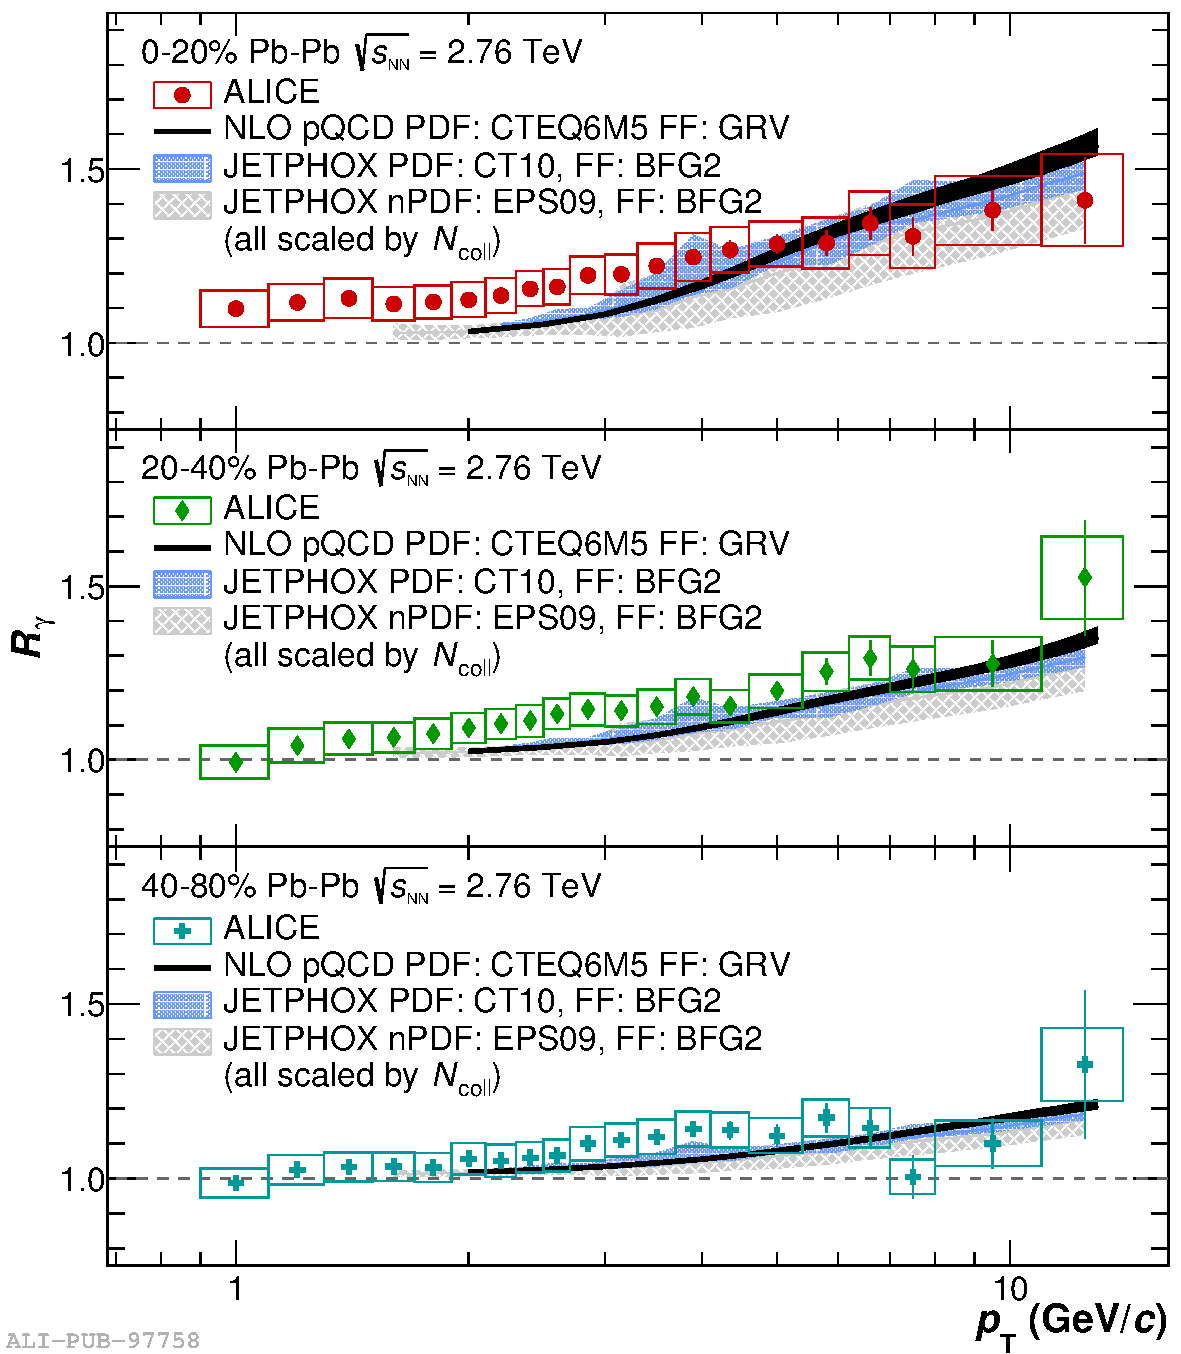
\includegraphics[width=0.46\textwidth]{\main/thermalradiation/figs/2015-Sep-24-DR_combMeasurement_incNLO.pdf}
\hfill
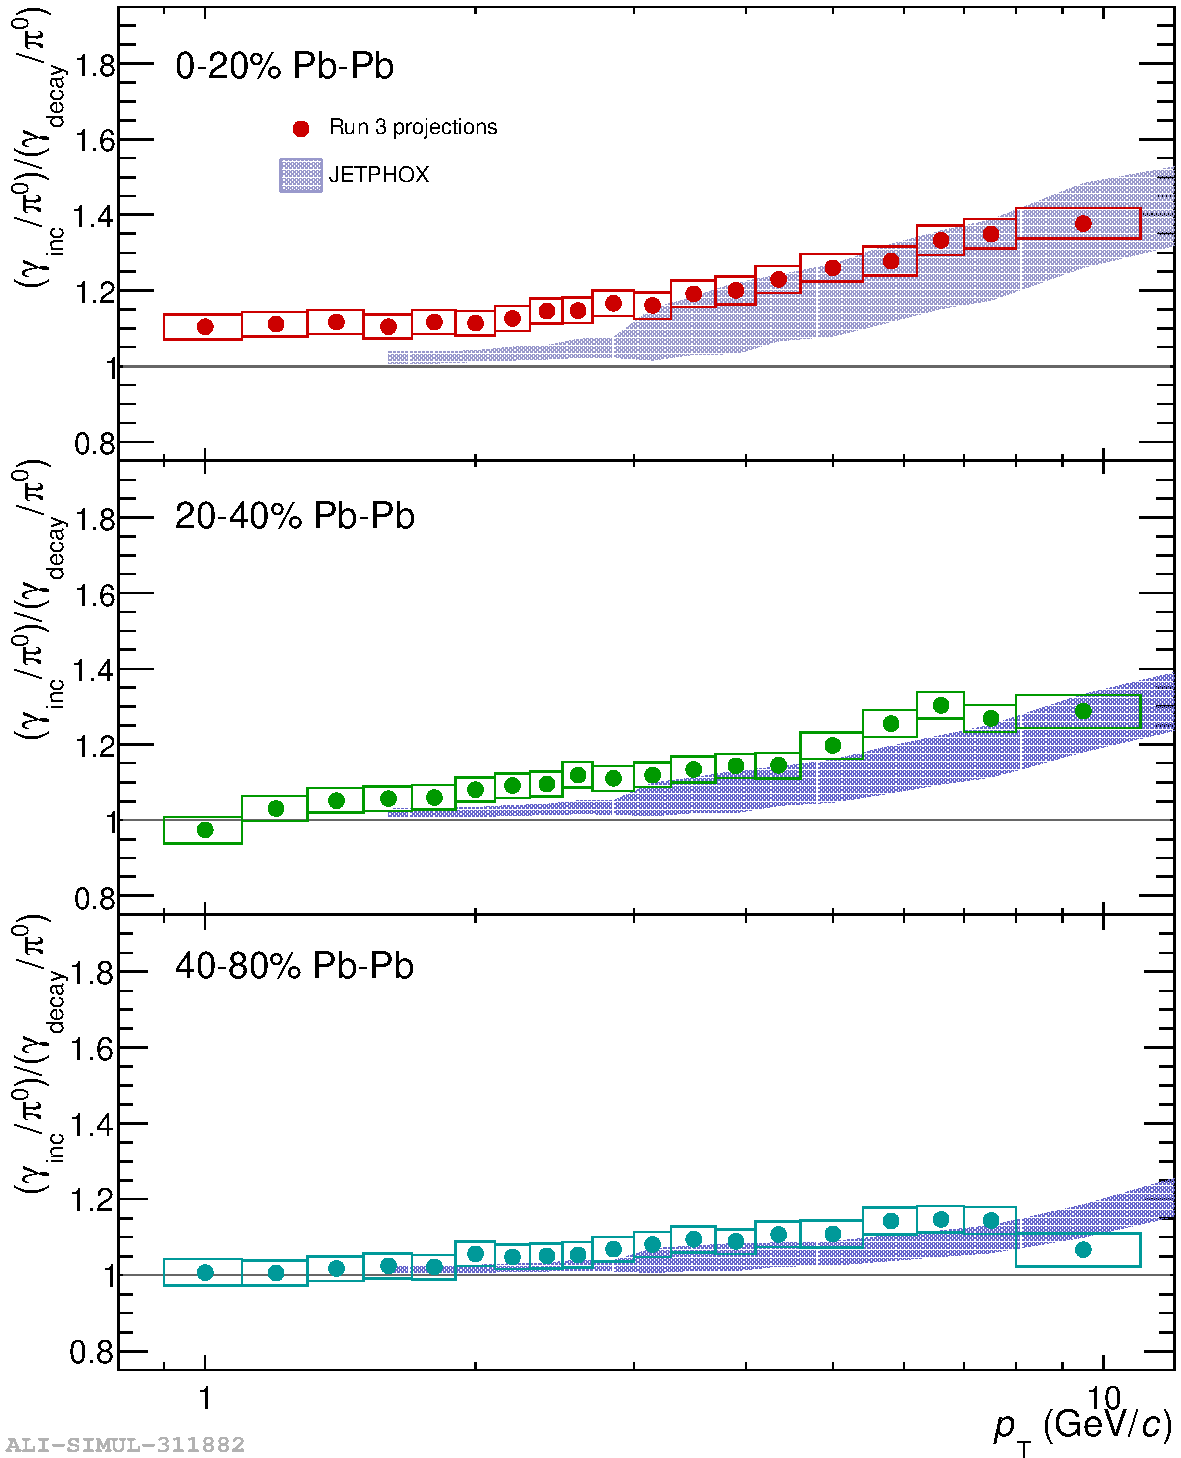
\includegraphics[width=0.425\textwidth]{\main/thermalradiation/figs/2018-10-10-2018-10-10-ReducedRg.pdf}
\caption{$R_{\PGg}$ measured \cite{Adam:2015lda} (left) and $R_{\PGg}$ projected keeping the measured values of $R_{\PGg}$ and recalculating the uncertainties as explained in the text.}
\label{fig:RealPhotonsRg}
\end{figure}
%-----------------------------------------------------------------------%

For Run 3 the PCM measurement will be influenced by the ALICE Inner Tracking System (ITS) and Time Projection Chamber (TPC) upgrades, while PHOS and the Electromagnetic Calorimeter (EMCal) will be kept unchanged. 
The new ITS shows an improved low \pT{} tracking efficiency and its material thickness is reduced by approximately 30\%. Two \unit[1]{\Umm} tungsten wires with well known thickness will be installed parallel to the beam direction. 
%The wires will be positioned between layers 2-3 and 4-5 at R = 4-14 cm and R = 30.9 cm, being inclined the most inner one. 
The TPC continuous readout mode together with large pile-up may prevent on the other hand the use of photon conversions beyond a radius of \unit[35]{\Ucm}. These will translate
into a ~35\% lower photon efficiency. On the other hand, the PCM measurement will also profit from the dedicated heavy-ion run with reduced magnetic field of the ALICE solenoid, that increases considerable the low \pT{} reconstruction efficiency.
To estimate how one can improve accuracy of our measurement, we split uncertainties into 3 classes: those which can be improved with increase of statistics (statistical uncertainties, uncertainties related to \PGpz spectrum extraction, $\PGh/\PGpz$ ratio); uncertainties which can be reduced using new techniques and some special methods (material budget estimate - with calibrated material analysis, energy scale in calorimeters with new hybrid \PGpz methods); and uncertainties related to the properties of the detector which can not be improved (hadron contamination in calorimeters, electron identification in conversion method etc.). To estimate the improvement of the uncertainties we assumed that the available statistics will increase by a factor of 100. 
%The main contributor to the systematic uncertainties at 
%low \pT\  for PCM is the material budget uncertainty with 4.5\%. 
The major improvement foreseen for Run 3 is the used of the calibrated tungsten wires
inserted in the ITS to determine the product of the photon flux times the \PGg reconstruction efficiency. This product would then be used to precisely determine the material thickness in the rest of the ITS (assuming $\varphi$-independent photon flux and taking the radial dependence of the reconstruction efficiency from simulation).
The proposed calibration method is based on weights calculated 
as the double ratio: 
\begin{equation}
\omega_i= 
{\left(\frac{N_{\PGg}^{\rm rec}(r_i)}{N_{\PGg}^{\rm rec}(r_{\rm wire})}\right)^{\rm data}} /
{\left(\frac{N_{\PGg}^{\rm rec}(r_i)}{N_{\PGg}^{\rm rec}(r_{\rm wire})}\right)^{\rm MC}} 
\end{equation}
where $N_{\PGg}^{\rm rec}(r_i)$ and $N_{\PGg}^{\rm rec}(r_{\rm wire})$ are the number of reconstructed \PGg 's in data or in MC simulations in a given radial bin and the calibrated wire, respectively.
%These weights are then used to scale the reconstruction efficiency in each radial bin of the detector.
This procedure is being implemented for Run 2 data using the TPC gas as calibration material. First results show that a systematic uncertainty of 1.8\% can be achieved. For the Run 3 projections a systematic uncertainty of 1\% on the ITS thickness is taken. The uncorrelated systematic uncertainties on the \PGpz and \PGh measurements will be reduced by a factor 10 due to the increased luminosity. The systematic uncertainties on photon selection and particle identification are expected to be reduced by 50\%.
Figure~\ref{fig:RealPhotonsRg} (right) shows the projection on the $R_{\PGg}$ measurement 
for Run 3 calculated with these assumptions: we keep measured values of $R_{\PGg}$ but re-calculate uncertainties. The total errors are reduced by $\sim50$\%. In addition to reductions of uncertainties, the large statistics foreseen for Run 3 will allow to explore the 0--1\% centrality. 

%{\bf Compare of different predictions Rg, with expected uncertainties: can we distinguish theories? Can we establish direct (thermal) photon measurements with 5 sigma? (Ana collect predictions and make Rg for 5 TeV, Cocktail: 5 TeV prelim pi0+eta/pi0 from 2.76)

%To which extend should we reduce sys/stat uncertainties to reach 5 sigma? Use our code.
%}

%Observation of the collective flow of final hadrons was one of the most important findings in the area of heavy-ion collisions.
%Collective flow is the azimuthal asymmetry in particle production, common for all soft particles in the collision. 
%It is interpreted as a collective expansion of initially spatially asymmetric hot matter. This initial deformation is the result of partial overlap of colliding nuclei in non-central collisions.  Transforming the initial geometric asymmetry into the asymmetry of momentum distribution of final particles requires strong interaction between particles of the matter, therefore hydrodynamic-like models provide very good description of this effect. 
%Direct photons do not interact with hot matter and deliver information about the collective  flow at the moment of their emission. As hydrodynamic models predict, photons emitted at the initial stage by hot quark-gluon matter carry very small collective flow since it is not developed yet at this stage. In contrast, direct photons emitted at the latest stage of hadron gas expansion carry much larger collective flow, similar to one of final hadrons. 
%Averaging over the whole history of the collision leads to the prediction of direct photon flow considerably smaller than one of final hadrons. 
%However, the first measurements of direct photon elliptic flow $v_{2}$ performed by PHENIX experiment \cite{Adare:2011zr}, demonstrated that the direct photon flow is comparable with one of final hadrons and much larger than one predicted by hydrodynamic models. 

%-----------------------------------------------------------------------%
\begin{figure}[htb]
\centering
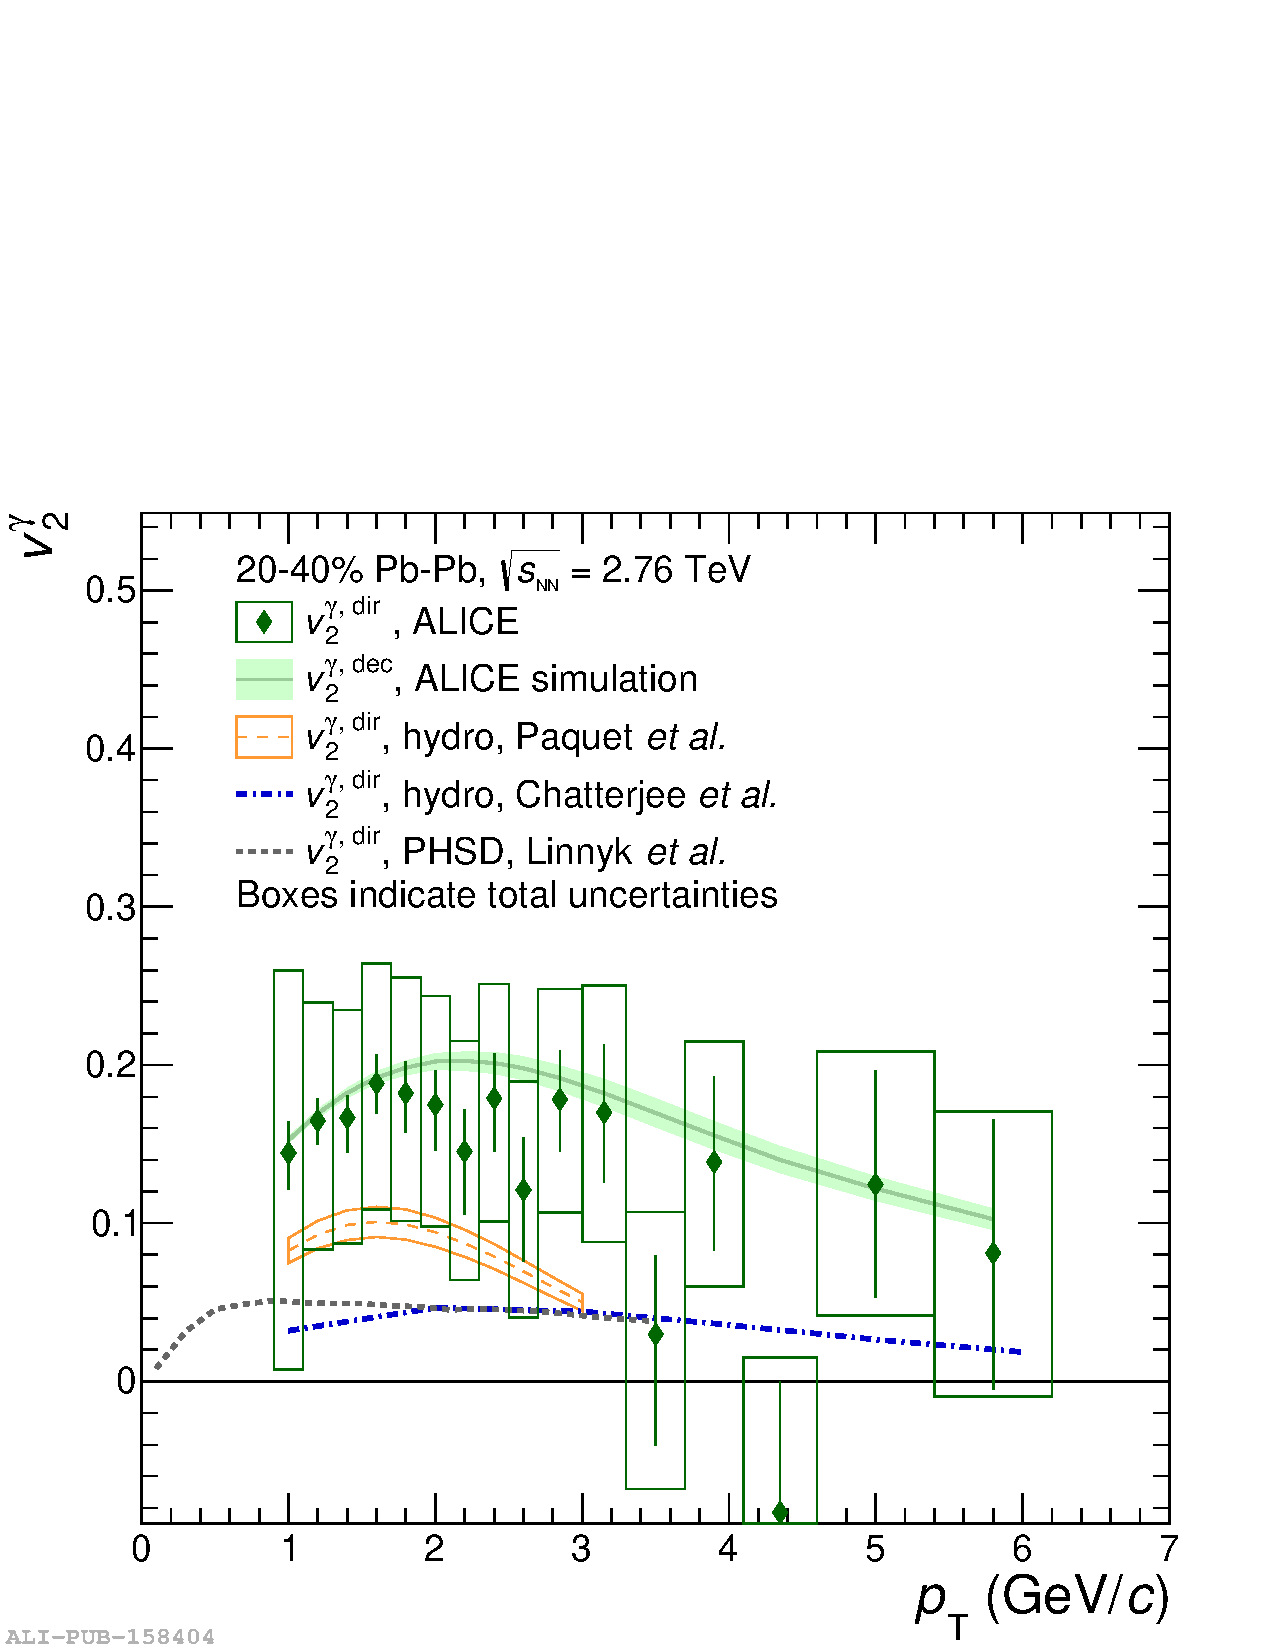
\includegraphics[width=0.45\textwidth]{\main/thermalradiation/figs/2018-May-11-2040_v2dir_combined_theory}
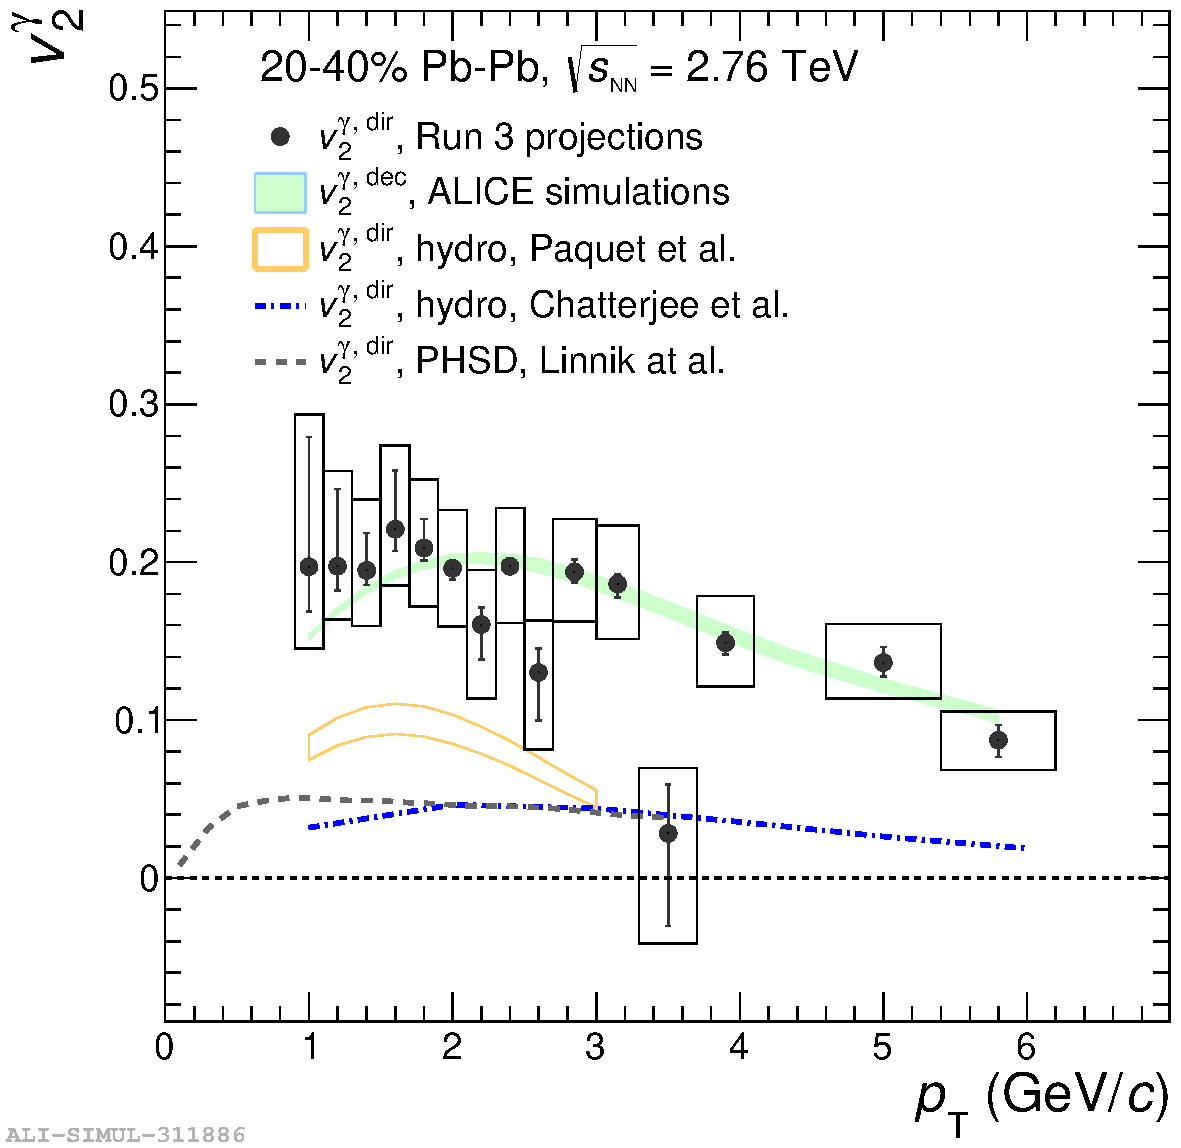
\includegraphics[width=0.42\textwidth]{\main/thermalradiation/figs/2018-10-10-2018-10-10-ProjectionV2.pdf}
\caption{Direct photon flow in mid-central collisions. Left: direct photon collective flow measured in \PbPb{} collisions compared to decay photon flow and several theoretical predictions. Right: expected accuracy in Run 3 keeping the  measured values of $R_{\PGg}$ and $v_{2}^{\PGg}$ and recalculating the uncertainties as explained in the text. }
\label{fig:RealPhotonsV2dir}
\end{figure}
%-----------------------------------------------------------------------%

ALICE performed measurements of the direct photon elliptic flow \cite{Acharya:2018bdy} in \PbPb{} collisions at $\sqrtsNN=\unit[2.76]{\UTeV}$ for the two centrality classes, 0--20\% and 20--40\%, see Fig.~\ref{fig:RealPhotonsV2dir}, left plot for 20--40\% centrality.
The measured direct photon elliptic flow $v_2^{\PGg,\rm dir}$ is compared to the estimated decay photon elliptic flow $v_2^{\PGg,\rm dec}$, marked as cocktail, and to the predictions of several theoretical models. Similar to RHIC measurements, the direct and decay photon elliptic flow are very close and systematically higher than theoretical predictions of hydrodynamic  \cite{Gale:2014dfa,Chatterjee:2017akg} and the transport  \cite{Linnyk:2015tha} models. However, because of the large uncertainties  one can not presently exclude neither of theoretical calculations. Using the same assumption concerning photon and neutral measurements in Run 3 as for $R_{\PGg}$, we estimated expected accuracy of $v_2^{\PGg,\rm dir}$ measurements in Run 3. We keep mean values the same but reduce uncertainties as expected, see Figure~\ref{fig:RealPhotonsV2dir} (right). shows the projection on the $v_2^{\PGg}$ measurement 
for Run 3. Similar to $R_{\PGg}$ with the current assumptions the total errors will be reduced by factor $\sim$ 2 and one will be able to exclude or confirm available theoretical calculations.
%{\bf We estimated v2dir with updated Rg uncertainties}





%\begin{itemize}
%\item First measurement at LHC from soft exponential component of photon pT spectrum (ALICE, Phys.Lett. B754 (2016) 235): T ~ 300 MeV (effective temperature averaged over system evolution)
%\item "Photon puzzle"
%\item Projections for Run3/4 in preparation: reduce systematic error (material budget uncertainty)
%\end{itemize}



\subsubsection{Dileptons}
\label{sec:thermalradiation:dileptons}
%Contributed by Raphaelle Bailhache, Oton Vazquez Doce, Michael Weber, Antonio Uras

The sensitivity to the expected signal of thermal radiation and an in-medium modification of the \PGr spectral function in the dielectron and dimuon channels with the ALICE detector \cite{Aamodt:2008zz,Abelev:2014ffa} was studied already in preparation for ITS upgrade in 2019/20 \cite{Abelevetal:2014cna,Abelevetal:2014dna,ALICE:2014qrd,ALICE:MFTLoI}. The measurement of low-mass dileptons after this upgrade will profit from  
\begin{itemize}
\item an improved vertex resolution, which leads to a better separation of electrons from prompt sources, like thermal radiation, and electrons from the decays of heavy-flavour hadrons, for which $c\tau$ is about \unit[150]{\Uum} (open-charm hadrons) or \unit[400]{\Uum} (open-beauty hadrons), 
\item a reduced material budget and improved tracking efficiency at low transverse momentum \pT, which leads to a smaller background of electrons and positrons from photon conversion in the detector material,
\item a higher rate capability (\unit[50]{\UkHz} in \PbPb{} collisions) that will increase the expected number of events in the central barrel detector by a factor of 100, 
\item a dedicated heavy-ion run with a reduced magnetic field of the ALICE solenoid ($B=\unit[0.2]{\UT}$ instead of \unit[0.5]{\UT}), which increases the phase-space acceptance and the reconstruction efficiency of low momentum particles 
\item and the installation of the muon forward tracker, that will lead to an improved mass resolution and reduced background in the dimuon channel.
\end{itemize}
The expected measured spectra discussed in this section closely follow the strategy that is discussed in more detail in \cite{Abelevetal:2014cna,Abelevetal:2014dna,ALICE:2014qrd,ALICE:MFTLoI}.

For the dielectron channel an integrated luminosity $\Lint\approx \unit[3]{\Unb^{-1}}$ is assumed, which should be collected in the dedicated \PbPb{} run at low field. The corresponding number of events in central (0--10\%) collisions is $2.5 \times 10^{9}$.  
The input for the signal is composed of:
\begin{itemize}
\item contributions from the decays of long-lived light pseudoscalar and vector mesons (hadronic cocktail consisting of \PGpz,\PGh,\PGh',\PGo, and \PGf), with particle ratios and spectral shapes extrapolated from existing heavy-ion data at lower energies,
\item correlated semileptonic charm decays based on calculations from the PYTHIA event generator \cite{Sjostrand:2006za},
\item and the radiation of thermal dileptons and a medium-modified spectral function for the \PGr meson in a realistic space-time evolution (see Fig.~\ref{fig:LHCExpectations_Rapp_pHSD}~(left)).
\end{itemize}
With respect to earlier calculations \cite{Abelevetal:2014cna,Abelevetal:2014dna,ALICE:2014qrd} we use here a fast simulation of central \PbPb{} collisions to estimate the combinatorial background and the statistical significance of the signal. The particles are produced with the event generator HIJING \cite{Wang:1991hta} and then propagated through the detector material by GEANT3 \cite{Brun:1994aa}. An updated geometry of the ITS is utilised in the detector description and leads to a more realistic treatment of conversion electrons and the subsequent background. 
Electrons are reconstructed and identified via signals in the ALICE Time Projection Chamber (TPC) and Time-Of-Flight (TOF) detector, a parametrised efficiency from runs at low magnetic field during LHC Run 2 is applied. After pairing electrons and positrons an additional selection on the pair distance of closest approach 
\begin{equation}
DCA_{ee}(\sigma)=\sqrt{(\mathrm{DCA}_{\mathrm{xy},1}/\sigma_{\mathrm{xy},1})^2+\mathrm{DCA}_{\mathrm{xy},2}/\sigma_{\mathrm{xy},2})^2}
\end{equation}
is applied to reduce the contribution from correlated semileptonic charm decays. The selection is chosen such that 95\% of these pairs are rejected, while having an efficiency for prompt pairs of $\sim17$\%.
The signal distribution $S$, which includes the remaining charm and beauty hadron decays, is obtained by subtraction of the combinatorial background from all \Pepem pairs. The combinatorial background $B$ is estimated from like-sign pairs and a correction factor $R$ that takes into account the different acceptance of the apparatus for unlike- and like-sign pairs \cite{Acharya:2018kkj,Acharya:2018ohw,Acharya:2018nxm}. The significance that is used to project the statistical uncertainty on the measurement is calculated as $S/\sqrt{S+2B}$. The signal S is shown in Fig.~\ref{fig:DileptonsSpectra}~(left) together with all input distributions. In order to extract the QGP component and the in-medium modified \PGr spectral function, the hadronic cocktail and the contribution from correlated semileptonic charm decays is subtracted and shown in Fig.~\ref{fig:DileptonsSpectraSubtracted}~(left). In addition, the systematic uncertainties from the combinatorial background and signal extraction, as well as physical backgrounds after subtraction are shown. The relative systematic uncertainty from tracking and track matching on the signal is assumed to be 4\%. For the systematic uncertainty on B a mass dependent uncertainty on the $R$ factor (0.2\% at $M_{\rm ee}=\unit[0.3]{\UGeVcc}$ \cite{Acharya:2018kkj}) is used. A relative systematic uncertainty on the light-hadron cocktail and on the total charm cross-sections of 10\% and 15\%, respectively, are applied.

In the dimuon channel, the full integrated luminosity of \PbPb collisions ($\Lint=10~\invnb$) is used. In this channel, the main source of background is represented by the combinatorial pairs of muons coming from uncorrelated semimuonic decays of light-flavoured mesons, mainly pions and kaons, copiously produced in high-energy nuclear collisions. The opposite-sign dimuon mass spectrum obtained after the subtraction of the combinatorial background evaluated by means of an event mixing technique, results from the superposition of several opposite-sign correlated dimuon sources, represented in the right panel of \figurename~\ref{fig:DileptonsSpectra}. 
% Vujanovic version
%In order to isolate the thermal dimuon radiation, which includes the in-medium modified line shapes of the $\PGr$ meson, 
%original version
In order to isolate the thermal dimuon radiation and the in-medium modified line shapes of the $\PGr$ meson,
the known and well-identifiable sources of the hadronic cocktail --- 2-body and Dalitz decays of the $\PGh$, $\PGo$, $\PGf$ mesons, for which no in-medium effect is expected --- are subtracted from the total opposite-sign correlated dimuon mass spectrum. A~10\% systematic uncertainty in the evaluation of the shape and the normalization of these sources has been considered in the performance studies. The same procedure has been also applied for the subtraction of the dimuons from the open charm and open beauty processes; alternatively, these two sources could be separated from the prompt ones by means of an analysis based on the discrimination of the dimuon offset at the primary vertex.



%-----------------------------------------------------------------------%
\begin{figure}[htb]
\centering
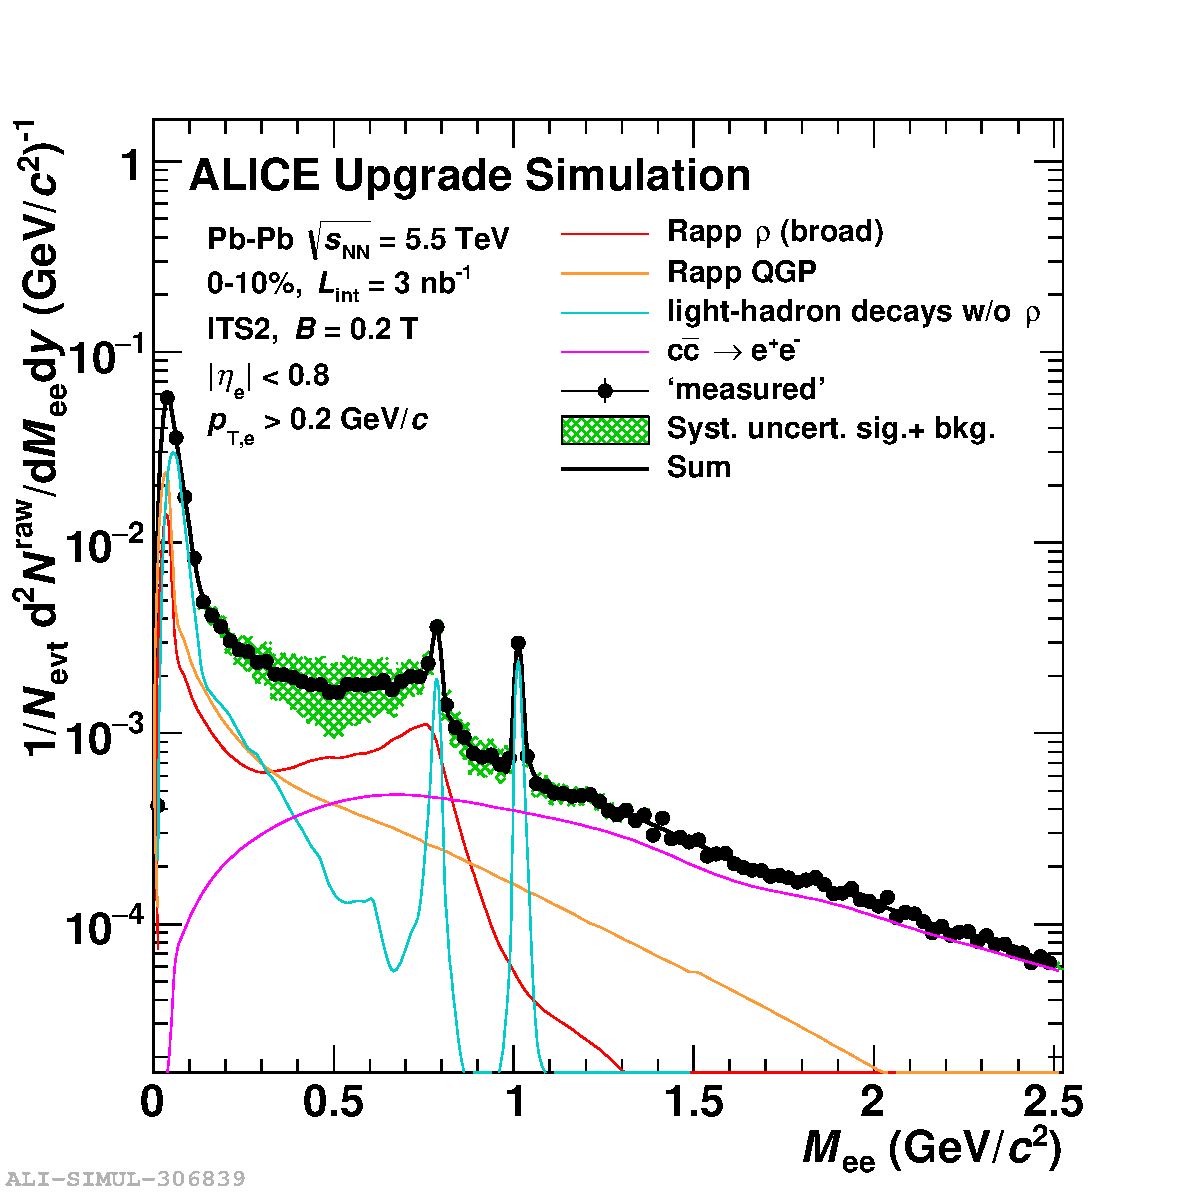
\includegraphics[width=0.45\textwidth]{\main/thermalradiation/figs/2018-10-21-2018-10-21-finalPlotsLowB_ITS3_EoI_final_Mee_ITSCyl0_IPcut1_events2500000000_redraw}
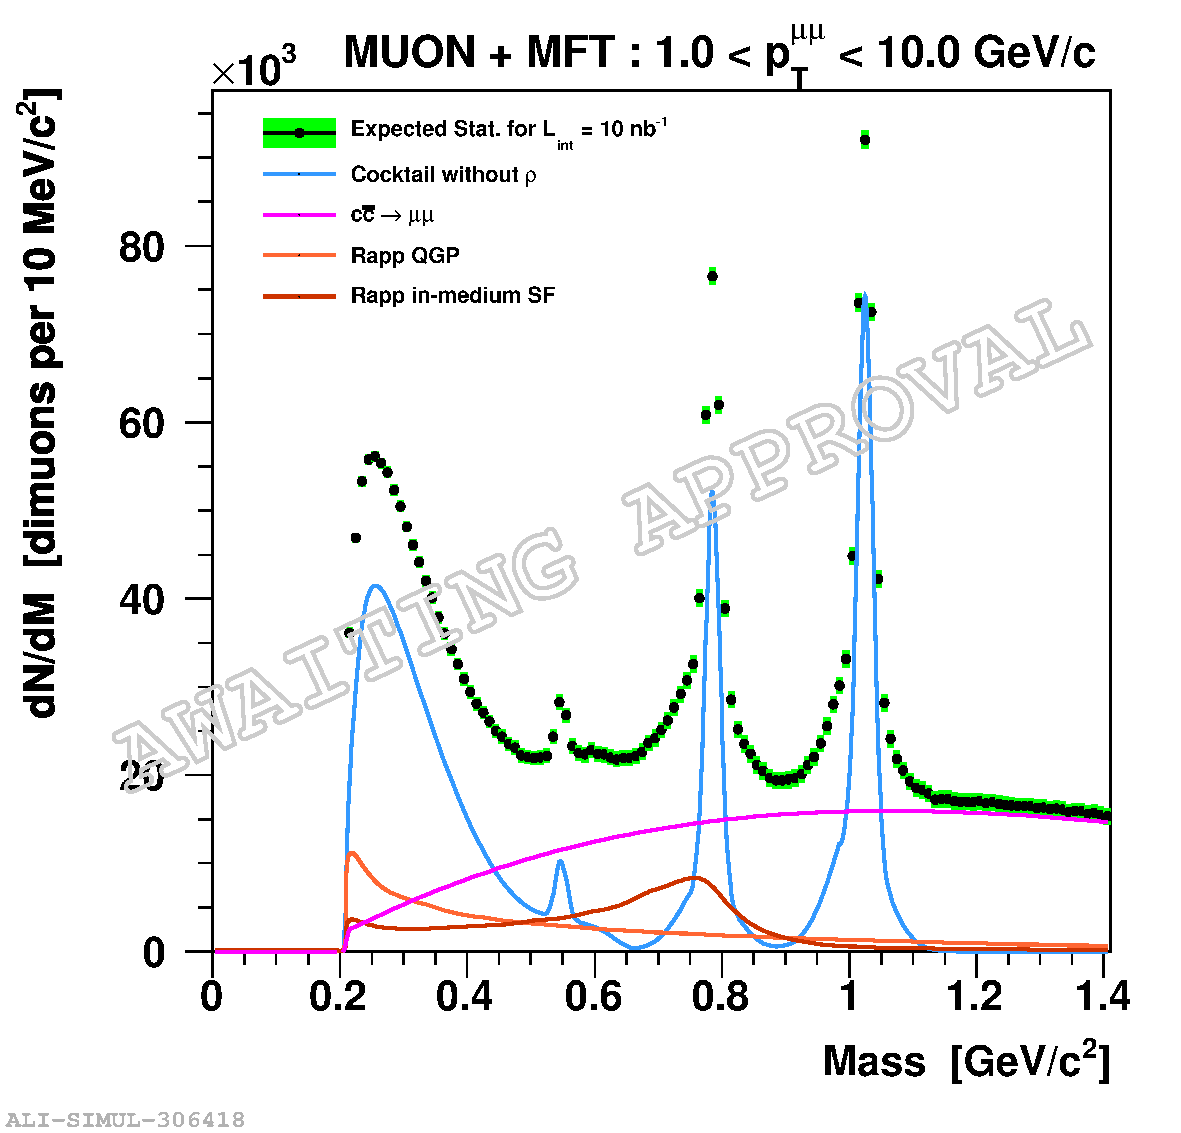
\includegraphics[width=0.45\textwidth]{\main/thermalradiation/figs/2018-09-14-2018-09-14-GlobalPlotLowMass_MFT_Pt_1_10}
\caption{Inclusive \Pepem (left) and \PGmpGmm (right) invariant mass spectrum for 0--10\% most central \PbPb{} collisions at $\sqrtsNN = \unit[5.5]{\UTeV}$. The green boxes show the systematic uncertainties from the combinatorial background subtraction.}
\label{fig:DileptonsSpectra}
\end{figure}
%-----------------------------------------------------------------------%

%-----------------------------------------------------------------------%
\begin{figure}[htb]
\centering
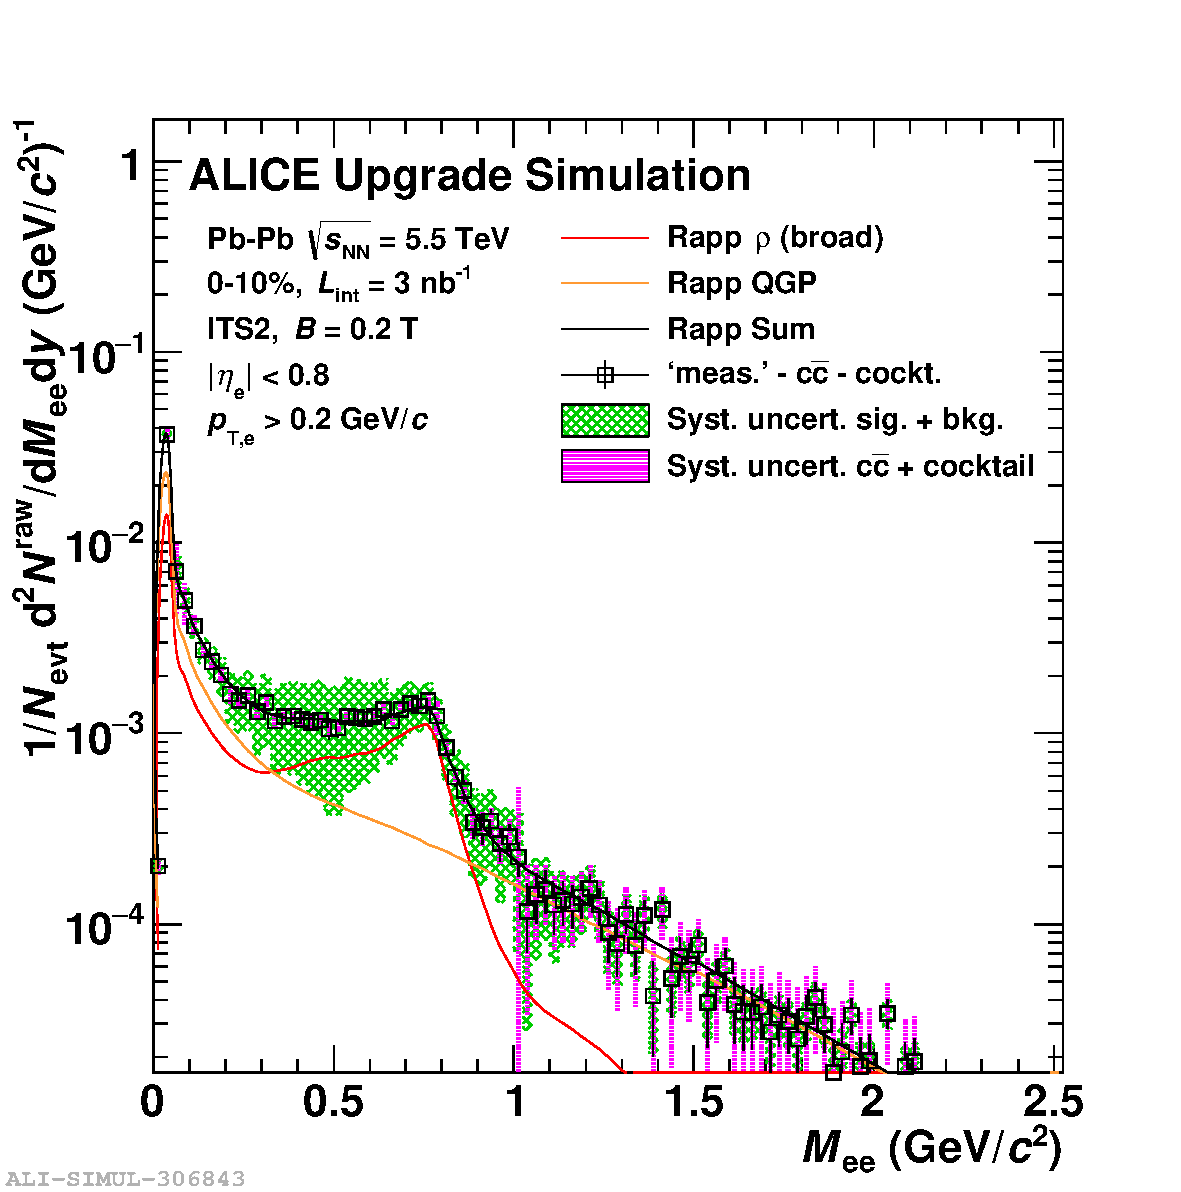
\includegraphics[width=0.45\textwidth]{\main/thermalradiation/figs/2018-10-21-2018-10-21-finalPlotsLowB_ITS3_EoI_final_Excess_ITSCyl0_IPcut1_events2500000000_redraw}
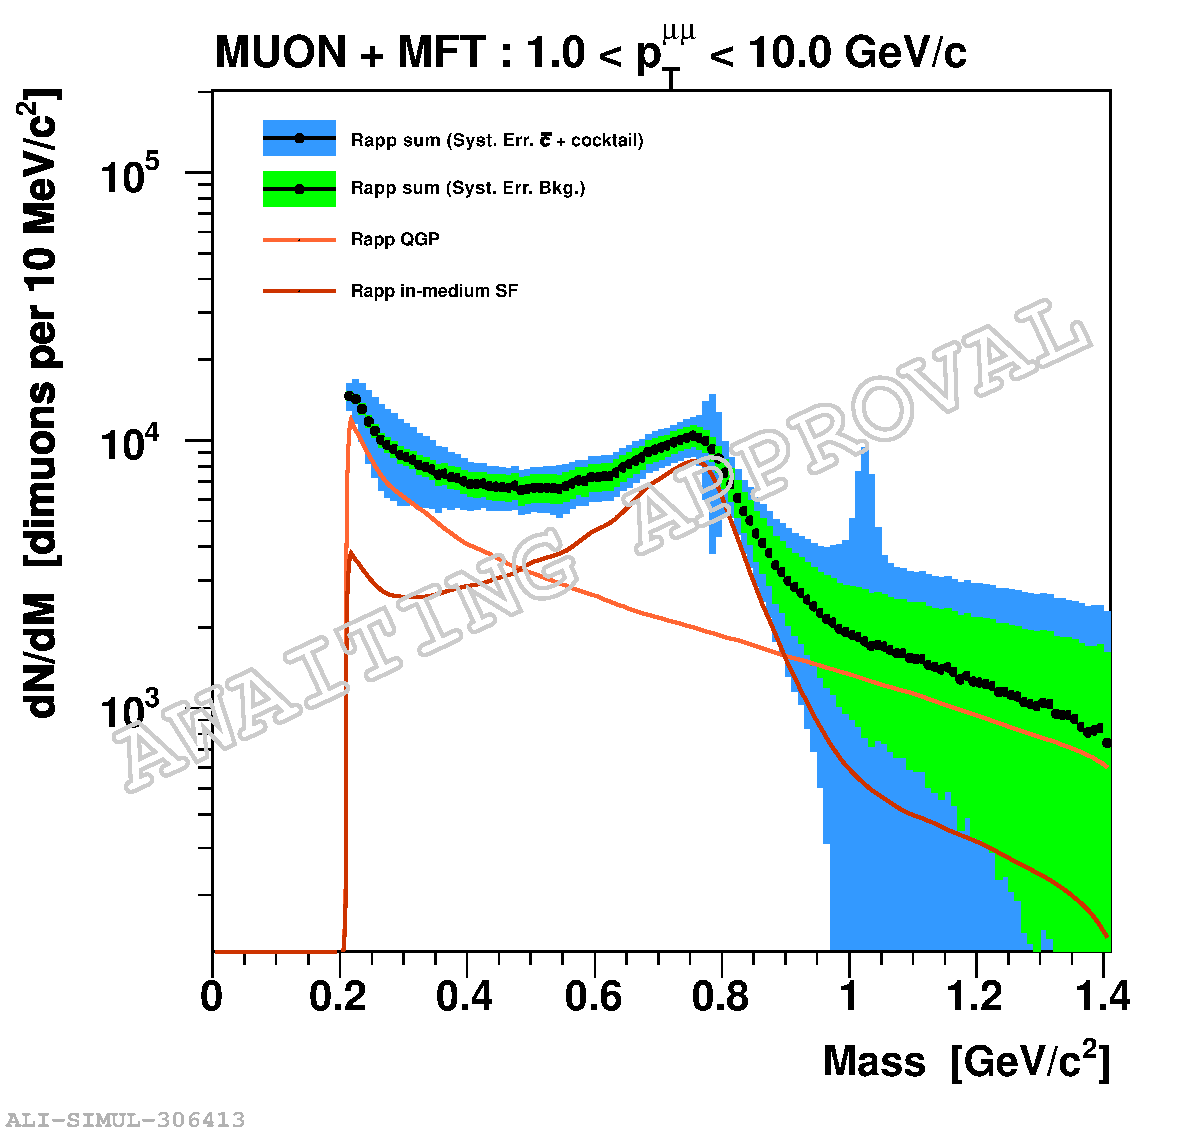
\includegraphics[width=0.45\textwidth]{\main/thermalradiation/figs/2018-09-14-2018-09-14-RappPredictionLowMass_MFT_Pt_1_10}
\caption{Excess (after subtraction of light hadron decays and from correlated charm semileptonic decays) \Pepem (left) and \PGmpGmm (right) invariant mass spectrum for 0--10\% most central \PbPb{} collisions at $\sqrtsNN = \unit[5.5]{\UTeV}$. The green boxes show the systematic uncertainties from the combinatorial background subtraction, the magenta (left) and blue (right) boxes indicate systematic errors related to the subtraction of the cocktail and charm contribution.}
\label{fig:DileptonsSpectraSubtracted}
\end{figure}
%-----------------------------------------------------------------------%

The spectral function of low-mass dielectrons and dimuons in the mass region of the modified \PGr-meson spectral function $M_{\rm ee}\approx\unit[0.5]{\UGeVcc}$ can be extracted with a systematic uncertainty of $\approx 40$\% and $\approx 20$\%, respectively (see Fig.~\ref{fig:DileptonsSpectraSubtracted}). 
The sizeable contribution of thermal dilepton pairs above $M_{\rm ee}>\unit[1.1]{\UGeVcc}$ can be used to extract the temperature of the system. An exponential fit with d$N$ /d$M_{\rm ee} \sim  M_{\rm ee}^{3/2}$ exp( - $M_{\rm ee} /T_{\rm fit}$ ) to the subtracted \Pepem spectra in the invariant mass region $1.1 < M_{\rm ee} < \unit[2.0]{\UGeVcc}$ was performed. Comparing the fit parameter $T_{\rm fit}$ to the real temperature $T_{\rm real}$ from the fit to the thermal contribution, a statistical uncertainty of 5\% and systematic uncertainty of 5\% and 20\% for the background and the charm subtraction, respectively, were estimated. The same kind of measurement is also expected to be possible in the dimuon channel, considering a dedicated set of cuts optimized for the analysis of the intermediate mass region mentioned above (the cuts considered in the right panel of \figurename~\ref{fig:DileptonsSpectraSubtracted} being optimized for the signal extraction in the mass region below $\sim \unit[1]{\UGeVcc}$).

An alternative method to separate the thermal component from the modified heavy-flavour production in the intermediate mass range, is to fit the measured $DCA_{ee}$ distribution as a function of the dielectron invariant mass and pair transverse momentum with a three component function, including the contributions from prompt dielectron sources, from open-charm hadron decays and from open-beauty hadron decays. Since the shape of the heavy-flavour $DCA_{ee}$ spectra is quasi model independent, the dielectron yield of open heavy-flavour decays in the ALICE acceptance can be determined from the data with small uncertainties, without relying on theoretical calculations. Such fits were performed already with the Run 1 data in \pp{} collisions at $\sqrts = \unit[7]{\UTeV}$ \cite{Acharya:2018ohw}. Nevertheless, the statistics available did not allow for a differential study.    

The measurement of the dielectron elliptic flow coefficient $v_2$ as a function of $M_{\rm ee}$ in peripheral \PbPb{} collisions (40--60\%) was studied already in \cite{Abelevetal:2014cna}. It was shown that an absolute statistical uncertainty on $v_2$ of $\sigma_{v_2} \approx 0.01$ can be achieved.

\subsection{Two-photon and photonuclear interactions}
\label{sec:dileptons:peripheral}
%Contributed by Spencer Klein

Although two-photon and photonuclear interactions are expected to occur in both ultra-peripheral (UPC) and more central collisions, they were not generally expected to be visible in non-UPC collisions.  The few final state particles from the photon-mediated interaction were expected to be swamped by the more copious hadronically produced particles.   That expectation changed recently, when ALICE \cite{Adam:2015gba} and then STAR \cite{Adam:2018tdm,Zha:2018ohg} and ATLAS \cite{Aaboud:2018eph} observed excesses of dileptons produced at very small pair \pT, $\pT < \unit[100]{\UMeVc}$.   These pairs were prominent in \PbPb{} and Au--Au collisions, but not in \pp{} interactions; the excess corresponded to $\Raa >5$ (sometimes much more, depending on the exact cut and centrality.  This is inconsistent with all expectations for hadroproduction, but  consistent with photoproduction, where the pair \pT{} scale is set by the nuclear radius $R_{\rm A}$, with $\pT \approx \hbar/R_{\rm A}$. 

UPC photon-mediated interactions have been studied at both RHIC and the LHC \cite{Baltz:2007kq,Bertulani:2005ru,Klein:2017nqo,Bertulani:1987tz,Baur:2001jj}.  The agreement between data and calculations is quite good.  Photoproduction of \PGr, \PGo, \PGr' , \PJGy, \PJGy', \PGU and direct \PGpp\PGpm pairs has been observed, along with two-photon production of dilepton pairs and light-by-light scattering.  In peripheral collisions, photon-mediated interactions might be used to probe the nuclear medium that they may occur in, including the QGP \cite{Aaboud:2018eph,Adam:2018tdm}. The produced leptons may interact with this medium, leading to alterations in their momentum.    

Peripheral collisions introduce several new considerations for  photon-mediated reactions, particularly evolving coherence conditions for both photon emission and coherent photon-nucleus scattering.  Photon emission in both $\PGg\PGg$ and photonuclear interactions is expected to be completely coherent, governed by the nuclear form factor $F(q)$ \cite{Vidovic:1992ik}.   The photon emission from a nucleus moving with Lorentz boost $\gamma$ should occur before the hadronic interaction (which is taken to occur at $t=0$), at a retarded time, $t-x/c$ \cite{Zha:2017jch}, where $x=|b|/\gamma$; $|b|$ is the transverse distance from the photon emission point to where it interacts. For very small impact parameters, some coherence may be lost, and a more detailed calculation is needed.  For photon-nucleus collisions, the situation is more complicated, and will be discussed below. 

Here, we discuss two-photon interactions and then coherent photonuclear interactions. 

\subsubsection{Two-photon interactions}

In two-photon interactions, each nucleus emits a photon, which then interact and form a lepton pair. In UPCs, this process is well described by the Weizs{\"a}cker-Williams approach (where each photon is treated as real), except at very low pair \pT, where a lowest-order QED calculation works better \cite{Adams:2004rz}. UPC calculations can be easily extended to include peripheral collisions \cite{Klein:2018cjh, Zha:2018ywo,Klusek-Gawenda:2018zfz}.  The kinematic distributions are similar to those in UPCs, and the cross-section depends on the range of impact parameters.

Recently, the ATLAS collaboration \cite{Aaboud:2018eph} presented results showing a dramatic modification to $\PGg\PGg\rightarrow\PGmpGmm$ in peripheral collisions.  Figure \ref{fig:ATLASacoplanarity} shows the pair acoplanarity $\alpha$, the azimuthal angular deviation from being perfectly back-to-back, and $A$, the energy imbalance between the two leptons.  For UPCs, they found good agreement with the STARlight \cite{Baltz:2009jk,Klein:2016yzr} reference, with the data and calculations peaked at small $\alpha$ and $A$.   More central collisions show dramatic changes with the low-$\alpha$ peak largely disappearing, and the $A$ distributions only minimally changed.  ATLAS described this as "Consistent with order of magnitude estimates from kinetic theory for multiple scattering off electric charges in thermal plasma."  Multiple scattering would remove the peak at low $\alpha$, but leave $A$ largely unaffected.  If multiple scattering is large, though, one also expects bremsstrahlung, which should increase $A$.   To evaluate this further requires a calculation of how many of the produced leptons are produced in the medium, and/or traverse it.  The STAR Collaboration has studied two-photon \Pepem production in peripheral Au--Au collisions; they found a small difference between their pair  \pT{} spectrum and calculations, and suggest that it might be due to medium effects\cite{Adam:2018tdm}. ALICE has not yet seen these pairs \cite{Adam:2015gba}, likely because their pair acceptance requires  lepton $\pT > \unit[1]{\UGeVc}$, eliminating most pairs from $\PGg\PGg$ reactions. 

Coupled with better theoretical calculations, HL-LHC can confirm and dramatically expand our understanding of this effect.   One important goal is to expand the study to cover a much wider range of masses.  Figure \ref{fig:project} shows the expected mass spectrum obtainable by ATLAS for a $\unit[13]{\Unb^{-1}}$ HL-LHC run, assuming no changes in the trigger; masses up to \unit[100]{\UGeVcc} should be accessible. These high mass pairs correspond to two-photon interactions in or very near the two nuclei, so should show increased effects due to interactions with the medium or magnetic fields associated with the Quark--Gluon Plasma. In contrast, lower masses correspond to larger distances between the dilepton production point and the nuclei, so in-medium effects may be smaller.  These lower masses should be accessible with a softer requirement on the muon momentum.   It would also be interesting to compare \Pepem with \PGmpGmm (and possibly \PGtp\PGtm), since the lighter leptons should interact more.  If the leptons interact with the medium, then the electron $A$ distribution should show more change than that for muons.  

\begin{figure}[htb]
\centering
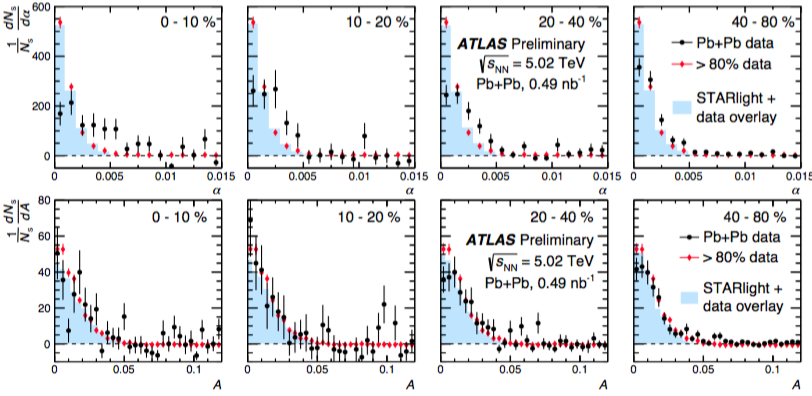
\includegraphics[width=0.85\textwidth]{\main/thermalradiation/figs/ATLASacoplanarity.png}
\caption{Acoplanarity ($\alpha$, top) and lepton energy imbalance ($A$, bottom) as a function of centrality, for dimuon pairs with pair mass above $\unit[10]{\UGeVcc}$, observed in the ATLAS detector.  From Ref. \cite{Aaboud:2018eph}.}
\label{fig:ATLASacoplanarity}
\end{figure}

\begin{figure}[htb]
\centering
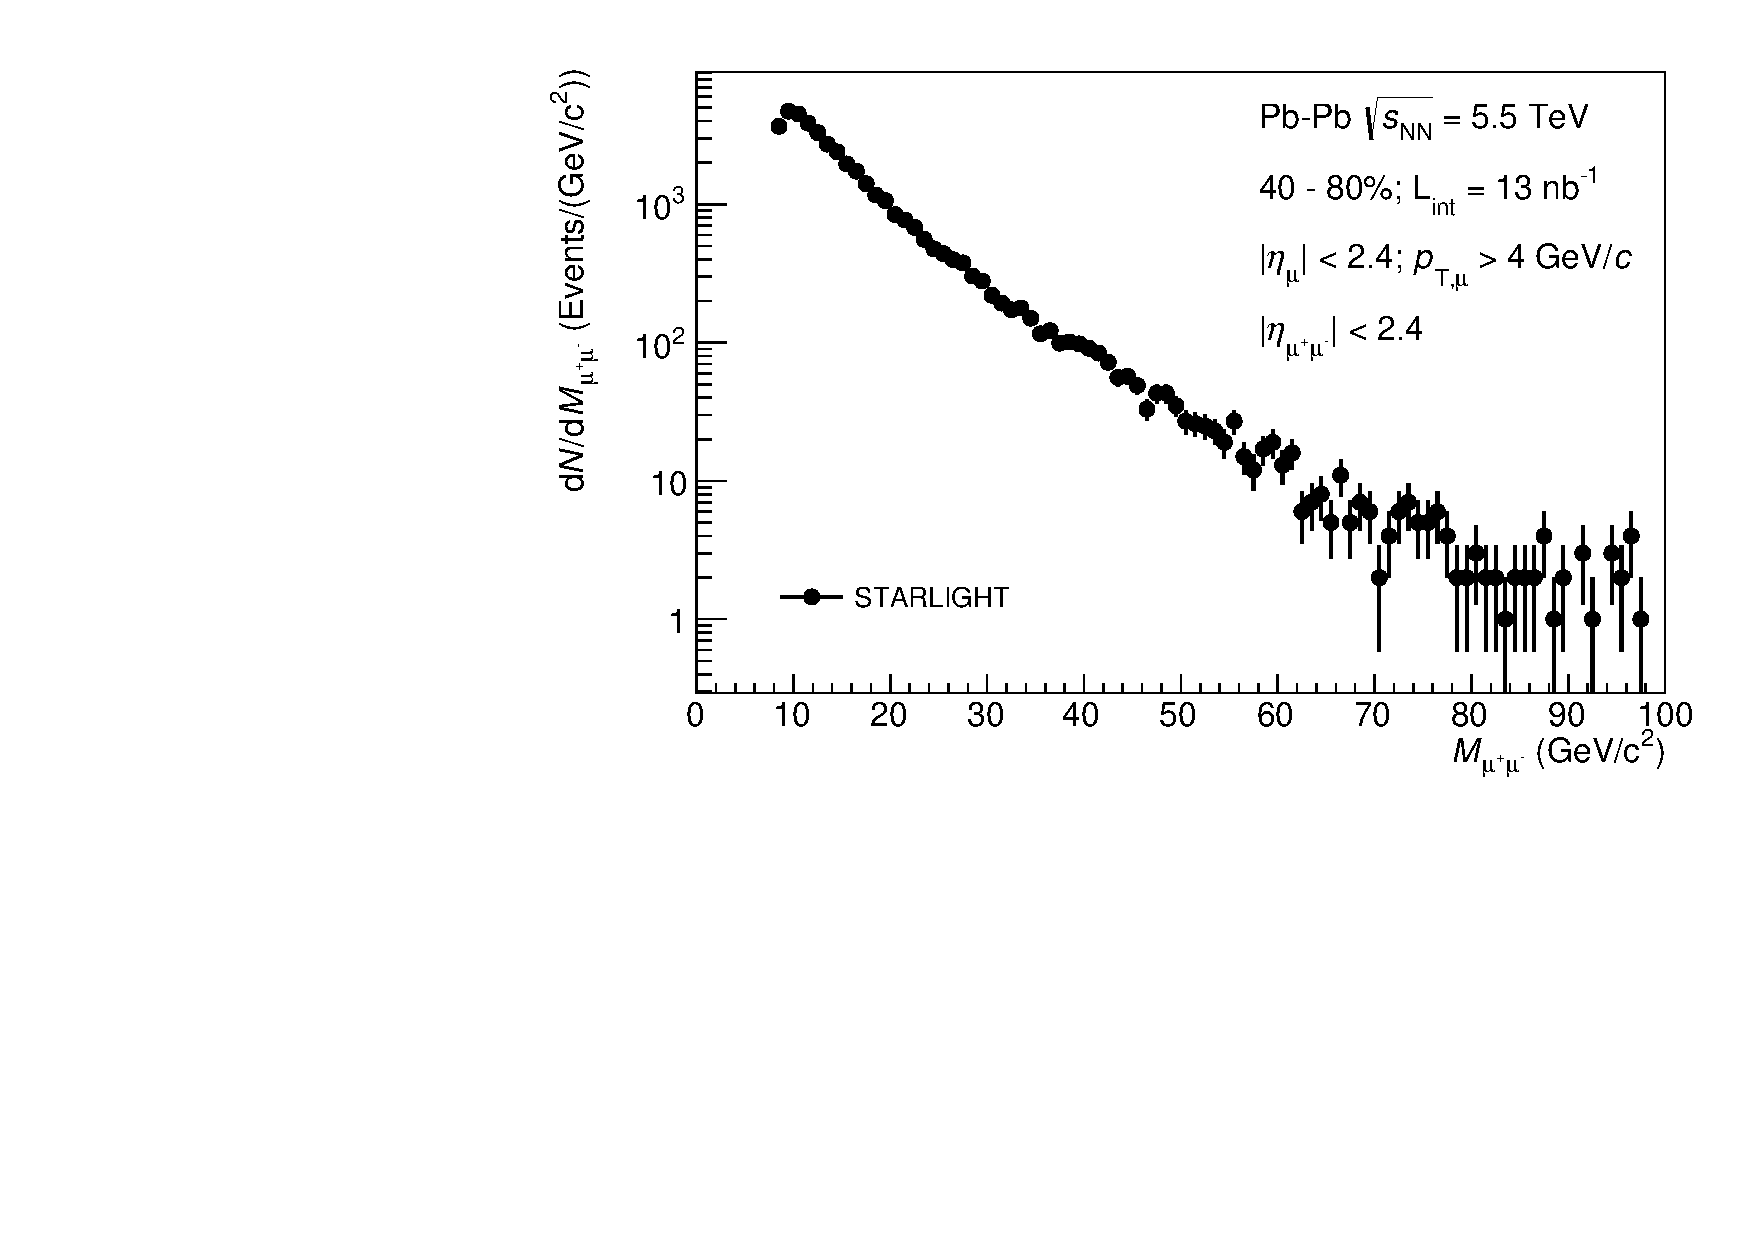
\includegraphics[width=0.5\textwidth]{\main/thermalradiation/figs/thermaldileptonmass_peripheralCollisions}
\caption{Expected dimuon yield in ATLAS acceptance (both muons with $\pT>\unit[4]{\UGeVc}$ and $|\eta|<2.4$), for 40--80\% centrality \PbPb{} collisions and the expected Run3/4 integrated luminosity of $\unit[13]{\Unb^{-1}}$.  Masses up to \unit[100]{\UGeVcc} are accessible.  The effective \unit[8]{\UGeVcc} minimum mass is because of the nearly back-to-back topology and the \unit[4]{\UGeVc} minimum muon \pT{} cut. This was calculated using STARlight \cite{Klein:2016yzr,Klein:2018cjh}.
}
\label{fig:project} 
\end{figure}


\subsubsection{Photonuclear interactions}

In photonuclear interactions, a photon emitted by one nucleus fluctuates to a quark-antiquark dipole, which then scatters elastically from the other (target) nucleus, emerging as a real vector meson.  The scattering occurs via Pomeron exchange, which preserves the photon quantum numbers.  In perturbative QCD, Pomerons are made up of gluons, so the process is sensitive to the gluon distribution in the target nucleus.  UPC measurements are consistent with moderate gluon shadowing.   In coherent scattering, the typical pair $\pT$ is $\hbar/R_{\rm A}$.  Incoherent scattering is also possible, with a lower cross-section.  There the quark-antiquark dipole scatters elastically from a single nucleon (or, at still higher $\pT$ inelastically from a single nucleon), producing a vector meson with a typical $\pT$ of a few hundred \unit[]{\UMeVc}.

Both ALICE \cite{Adam:2015gba}  and STAR \cite{Zha:2018ohg} have observed coherent \PJGy photoproduction in peripheral heavy-ion collisions.  There are a number of parallel theoretical calculations \cite{Klusek-Gawenda:2015hja,Zha:2017jch}.  The photon emission process is similar to the two-photon case, but the dipole-nucleons scattering happens at the same time as the hadronic interaction, introducing several complications to the calculations.  This immediately raises several questions:  What happens to the coherence if a target nucleon is involved in an interaction?   Does the dipole-nucleon interaction occur before or after the nuclear collisions?    If the hadronic interaction occurs first, the target nucleon will have lost energy, so the photon-nucleon cross-section will be smaller.  A detailed calculation should consider both possibilities.   There is also destructive interference between photoproduction from the two possible target nuclei \cite{Abelev:2008ew}; this interference extends to higher $\pT$ for more central collisions, and should reduce the cross-section for the region where nuclear collisions occur. At $b=0$, we expect complete destructive interference.  Ref. \cite{Zha:2017jch} makes predictions for a variety of coherence conditions, and as Fig. \ref{fig:jpsiinpcs} shows, finds that the ALICE and STAR data likely lie below the region where there is complete coherence for both photon emission and scattering, but probably above that where coherence is limited to only the spectator nucleons.  This is not surprising, but there is at least one element missing from this calculation. The lifetime of \PJGy particles is of the order $\unit[10^{-20}]{\Us}$, far shorter than that of the expanding Quark--Gluon Plasma.  Coherently photoproduced \PJGy have $\pT \sim \unit[100]{\UMeVc}$, so, near mid-rapidity,  are moving at a small fraction of the speed of light.  Particularly for more central collisions, one would expect many of them to be engulfed by the expanded QGP, before they have a chance to decay.  

The ALICE error bars are large, and more data, from the current runs and HL-LHC is needed to pin down the centrality dependence of the cross-section.  More data will also allow access to additional observables.  A detailed study of the shape of d$\sigma/$d$|\pT|$ would shed more light on the possible loss of coherence in more central collisions. There are also expected correlations between the reaction plane, which can be determined from the hadronic part of the collision, with the photonuclear interaction.  Because the destructive interference between photoproduction at mid-rapidity on the two nuclei goes as $\sigma \sim |1-\exp{(i{\vec{b}\cdot\vec{\pT})}}|^2$ \cite{Klein:1999gv}, the azimuthal direction of $\vec{\pT}$ provides information about the azimuthal direction of $\vec{b}$, \ie the reaction plane.  Thus, it can be used either as an independent measurement of the reaction plane, or as a test of the loss of correlation.  Also, the \PJGy polarization follows that of the photon that produced it, so it also follows $\vec{b}$, providing another probe of the reaction plane.  With a large data sample, we may also be able to probe incoherent \PJGy photoproduction, at least in very peripheral hadronic collisions, where the signal-to-noise ratio is high.  

It would also be very interesting to study \PGy' and \PGU photoproduction in peripheral collisions.  Since these mesons have different sizes from the \PJGy, they should interact with the medium with different strengths.  These studies should be possible at HL-LHC.  

\begin{figure}[htb]
\centering
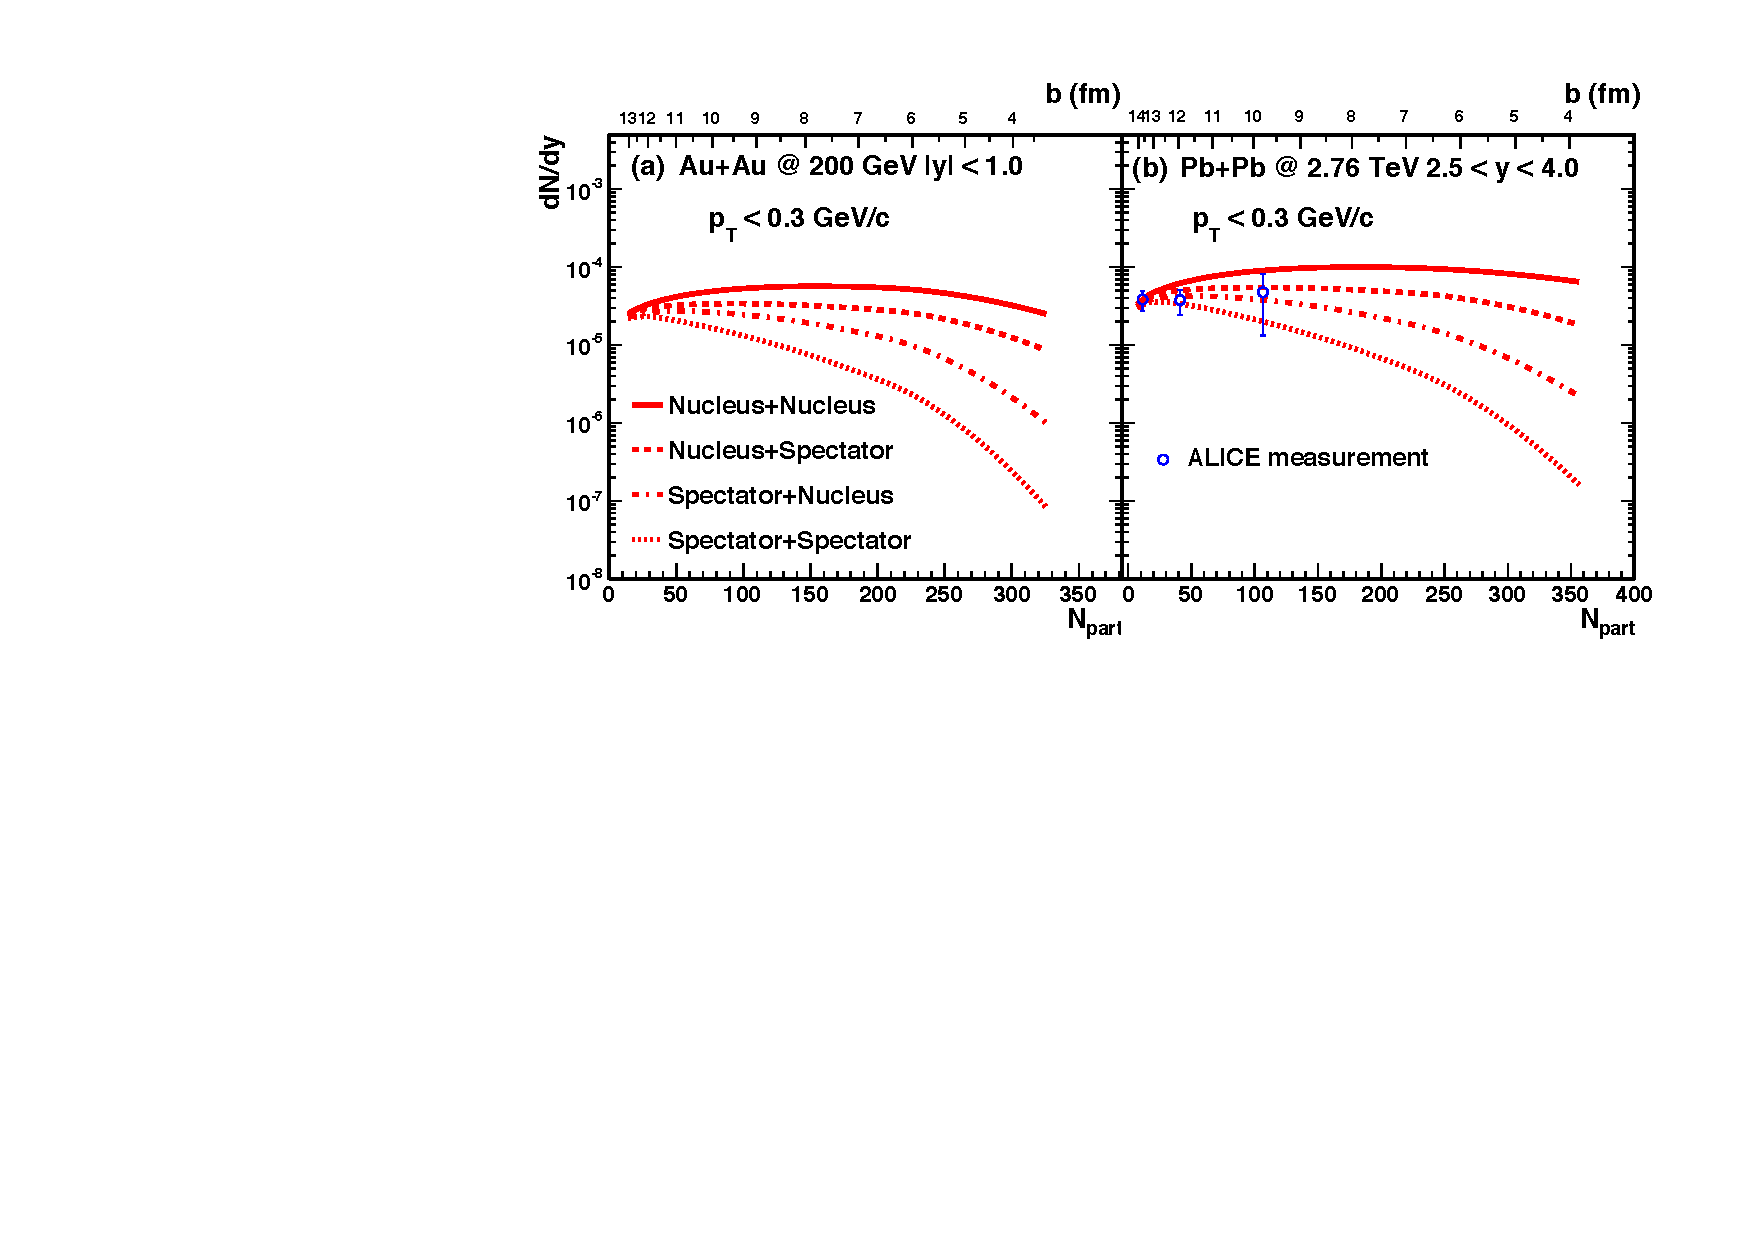
\includegraphics[width=0.85\textwidth]{\main/thermalradiation/figs/jpsiinpcs.pdf}
\caption{$J/\psi$ coherent photoproduction cross-sections in peripheral collisions, as a function of the number of participants (bottom), and impact parameter (top) with Au--Au collisions at RHIC (left) and \PbPb at the LHC (right).  The four curves are for different assumptions regarding centrality for the photon emitter (first particle listed) and the target (second particle listed).  From Ref. \cite{Zha:2017jch}.}
\label{fig:jpsiinpcs} 
\end{figure}


\subsection{Dark photons}
\label{sec:dileptons:darkphotons}
%Taku Gunji
% ------ dark photon section written by T. Gunji ------ %

Dark Matter is a hypothetical form of matter that is responsible for accounting for approximately 80\% of the matter in the Universe~\cite{Planck:2013jfk}.
Dark matter cannot be incorporated into the Standard Model, so the introduction of dark matter requires new interactions between dark matter particles 
and the ordinary Standard Model particles via unknown dark-sector forces~\cite{Alexander:2016aln}. 
The dark sector could have a rich structure with a few possible candidates, 
where one of them is regarded as Dark Photon ($A'$) with 
$L_{mix} \propto\frac{g}{2}F^{\mu\nu}X_{\mu\nu}$.
%Axion type known as Axion-like particles (ALPs) ($\frac{a}{f_a}F^{\mu\nu}\tilde{F}_{\mu\nu}$), Vector type regarded as Dark Photon ($A'$) ($\frac{g}{2}F^{\mu\nu}X_{\mu\nu}$), 
%Higgs type as dark scalar ($g_{H}|h|^2|\phi|^2$), and Neutrino type known as sterile neutrino ($g_{\nu}(hL)\psi$).
The dark photon is introduced as an extra-$U(1)$ gauge boson and acts as a messenger particle of a dark sector 
with the residual interaction ($g$) to the Standard Model particles.
%In the simplest scenario, where the coupling arises from the kinematic mixing interaction, 
%mixing parameter ($g$) is estimated to be in the rage of $10^{-4}$ -$10^{-2}$ at the one-loop level.
Understanding of possible interactions of dark photons has been motivated by 
a number of astrophysical anomalies such as antiproton spectrum in 
the cosmic rays measured by AMS Collaboration,
positron excess in the cosmic rays observed earlier by PAMELA~\cite{Adriani:2008zr}
and confirmed by FERMI~\cite{FermiLAT:2011ab} and AMS~\cite{Aguilar:2013qda}, 
and the long standing discrepancy
between the measured and the calculated anomalous magnetic moment of 
the muon $(g-2)_{\mu}$, where
the difference is more than three standard deviations away from zero~\cite{Bennett:2006fi}.

%Further constraints of dark photon mass ($m_{A'}$) and mixing parameter ($g$) have been 
%performed recently by beam-dump experiments ()~\cite{} , fixed-target experiments~\cite{} , 
%and collider experiments~\cite{} . 

%Figure~\ref{fig:darkphoton2016} shows 
%compilation of existing Dark Photon constraints in ($m_{A'}$, $g$ ) in 2016.

If the dark photon is the lightest state of the dark sector 
and therefore can decay only into the Standard Model particles, dark photons with mass $m_{A'} \le 2m_{\mu}$ decay only into electron-positron pairs. 
For dark photons above 2 muon threshold ($m_{A'} \ge 2m_{\mu}$), 
dark photons can decay into muon pairs. For ($m_{A'} \ge 2m_{\pi}$), 
dark photons can decay into hadrons as well. 
A lot of experimental activities have been seen recently 
and constraints of mixing parameter ($g^2$) as a function 
of dark photon mass ($m_{A'}$) has been done from many experiments. 
They are, for example, 
%\todo{missing reference in the caption}{Figure}~\ref{fig:darkphoton2016} shows compilation of existing Dark Photon constraints in ($m_{A'}$, $g$ ) in 2016, where they are from 
beam-dump experiments (measurement of lepton pairs from dark photons 
behind a sufficiently long shield. 
Examples are E141~\cite{Riordan:1987aw} and E137~\cite{Bjorken:1988as}
at SLAC, E774~\cite{Bross:1989mp} at Fermilab), 
fixed-target experiments (by scattering the electron beam on a nuclear target, 
the dark photon may be emitted in the initial or final state and coupling to 
electron-positron pairs is studied by looking for a bump in the 
electron-positron invariant mass. Examples are A1~\cite{Merkel:2014avp} 
at MAMI in Mainz, APEX~\cite{Abrahamyan:2011gv} at JLAB, 
DarkLight~\cite{Balewski:2013oza} at JLAB)
and collider experiments (BABAR~\cite{Lees:2014xha}, 
NA48/2~\cite{Batley:2015lha} at SPS, WASA~\cite{Moskal:2014dsa} at COSY, 
HADES~\cite{Agakishiev:2013fwl} at GSI, 
PHENIX~\cite{Adare:2014mgk} at RHIC, LHCb~\cite{Aaij:2017rft} and ALICE at LHC).
Since any process in which a virtual photon couples to lepton pairs or hadrons 
can be used to search for dark photons, 
following processes are used in the collider experiments: measurements of Dalitz decays of the $\PGpz/\PGh/\PGh' \rightarrow \PGg A'$ mesons and rare meson decays such as $\PK\rightarrow \PGp A'$, $\PGf \rightarrow \PGh A'$, 
and $\PDst \rightarrow \PDz A'$,
Bremsstrahlung process 
($\Pem Z \rightarrow \Pem ZA'$ with $A'$ emitted at very forward direction),  
radiative decay of vector resonances and initial state radiation 
(done by BABAR using radiative decays of $\PGUP{3S}$ and 
done by KLOE~\cite{Archilli:2011zc} using $\PGf \rightarrow \Pepem$).
%firstly explored by BABAR that looked for the bumps in the invariant mass spectrum of muon pairs in radiative decays of $\Upsilon(3S)$ and 
%later done by KLEO using $\phi \rightarrow e^+e^-$), 
%and initial state radiation (done by KLEO that searched for peaks 
%in muon pairs and electron pairs below 1 GeV and probed by BABAR below 10 GeV.). 
%New paragraph from IceCube 
%
%Ardid:2017lry
The 79-string IceCube search for dark matter in the Sun public data is 
used to test Secluded Dark Matter models~\cite{Ardid:2017lry}. 
Dark matter particles can be captured by the Sun, annihilate, and 
produce a neutrino flux that can be observed at Earth and that 
depends on the dark matter scattering cross section off nuclei
and on the dark matter annihilation rate and final states.
This analysis constrains a kinetic mixing parameter $g \sim 10^{-9}$
between 0.22 and $\sim\unit[1]{\UGeV}$~\cite{Ardid:2017lry}.

%\begin{figure}[htb]
%\centering
%\includegraphics[width=0.65\textwidth]%{\main/thermalradiation/figs/darkphoton2015.png}
%\caption{Constraints in the $g$ vs. $m_{A'}$ planes for dark photons. From \cite{reference}.}
%\label{fig:darkphoton2016}
%\end{figure}

%\subsubsection{Constraints by ALICE and LHCb from Run1 and Run2 data}
ALICE has good capabilities for electron identification in the low 
transverse momentum region, that enables the measurement of a large sample of 
the \PGpz Dalitz decays~\cite{Acharya:2018ohw}. 
ALICE searches for possible decays of 
$\PGpz \rightarrow \PGg A', A' \rightarrow \Pepem$ 
by examining the electron-positron invariant mass in a large sample
of \PGpz Dalitz decay for $20 \le M_{\rm ee} \le \unit[90]{\UMeVcc}$ in 
\pp{} collisions at \unit[7]{\UTeV} ($\Lint \sim \unit[4]{\Unb^{-1}}$) and 
\pPb{} collisions at \unit[5.0]{\UTeV} ($\Lint \sim \unit[40]{\Uub^{-1}}$) as shown in 
%from Run 1~\cite{} , where 90\% of CL of $g^2$ is shown in 
Fig.~\ref{fig:darkphoton_alice_lhcb}.\\
LHCb has good capabilities to measure muons and hardware and software 
triggers enable the accumulation of a large sample of dimuon pairs. 
LHCb searches for prompt-like and long-lived dark photons 
produced in \pp{} collisions at \unit[13]{\UTeV}, using $A' \rightarrow \PGmpGmm$ decays 
from a large data sample corresponding to $\Lint \sim \unit[1.6]{\Ufb^{-1}}$ 
collected during 2016, where 
the prompt-like $A'$ search is shown in Fig.~\ref{fig:darkphoton_alice_lhcb}~\cite{Aaij:2017rft}.
%The prompt-like $A'$ search is performed 
%from near the dimuon threshold up to 70 GeV, while the long-lived $A'$
%search is restricted to the mass range 214 $\le m(A') \le 350$ MeV.
%Result of 90\% of CL of $g^2$ for prompt-like $A'$ 
%is shown in Fig.~\ref{fig:darkphoton_lhcb}.

\begin{figure}[htbp]
\begin{center}
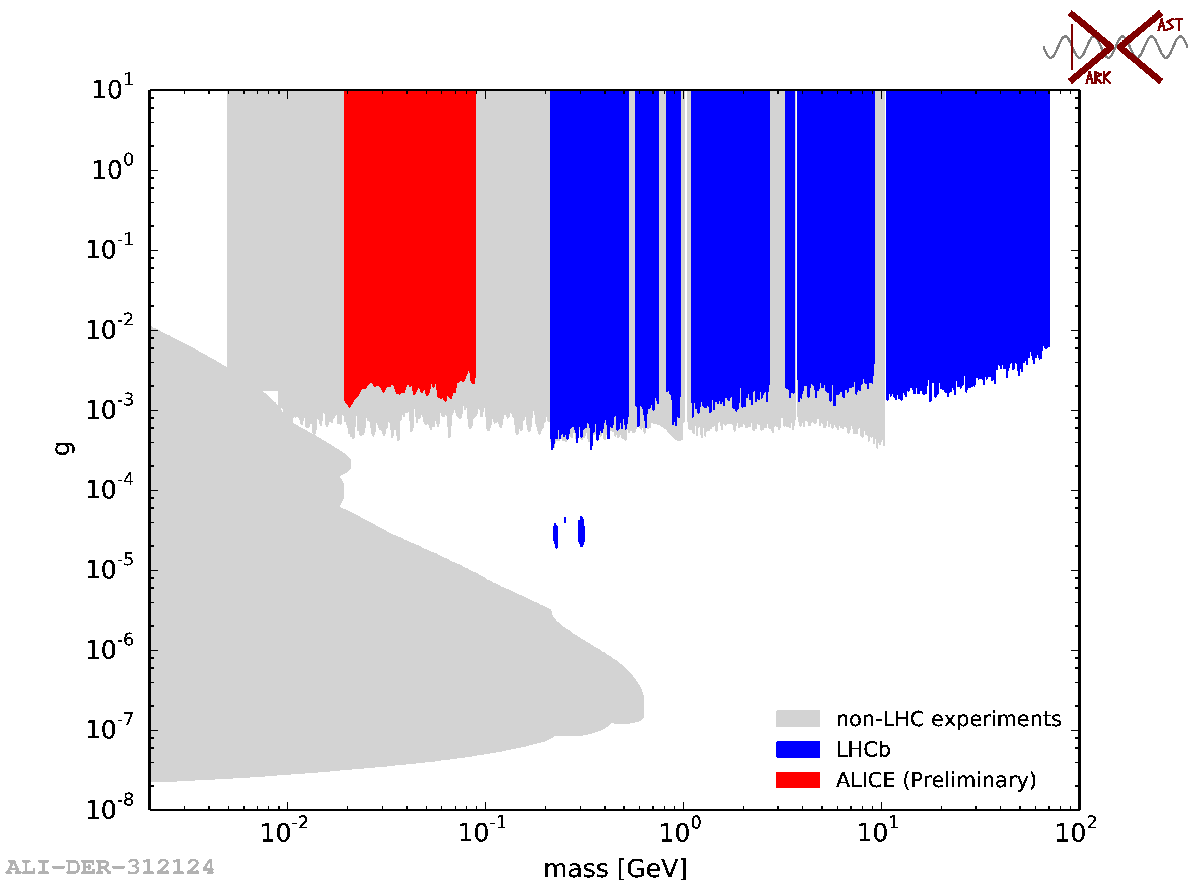
\includegraphics[width=120mm]{\main/thermalradiation/figs/2018-10-21-2018-10-21-2018-10-21-visible2}
\end{center}
\caption{90\% of confidence level of mixing parameter as a function of dark photon mass. Figure is adapted from Ref.~\cite{Ilten:2018crw}. 
Red and blue are from ALICE and LHCb~\cite{Aaij:2017rft}. 
Light grey band contains results from BABAR, KLOE, A1, APEX, NA48/2,  E774, E141, E137, KEK, Orsay, BESIII, CHARM, HPS, NA64, NOMAD, NuCAL, and PS191~\cite{Ilten:2018crw}.}
\label{fig:darkphoton_alice_lhcb}
\end{figure}
 
%\begin{figure}[htbp]
% \begin{minipage}{0.5\hsize}
%  \begin{center}
%%   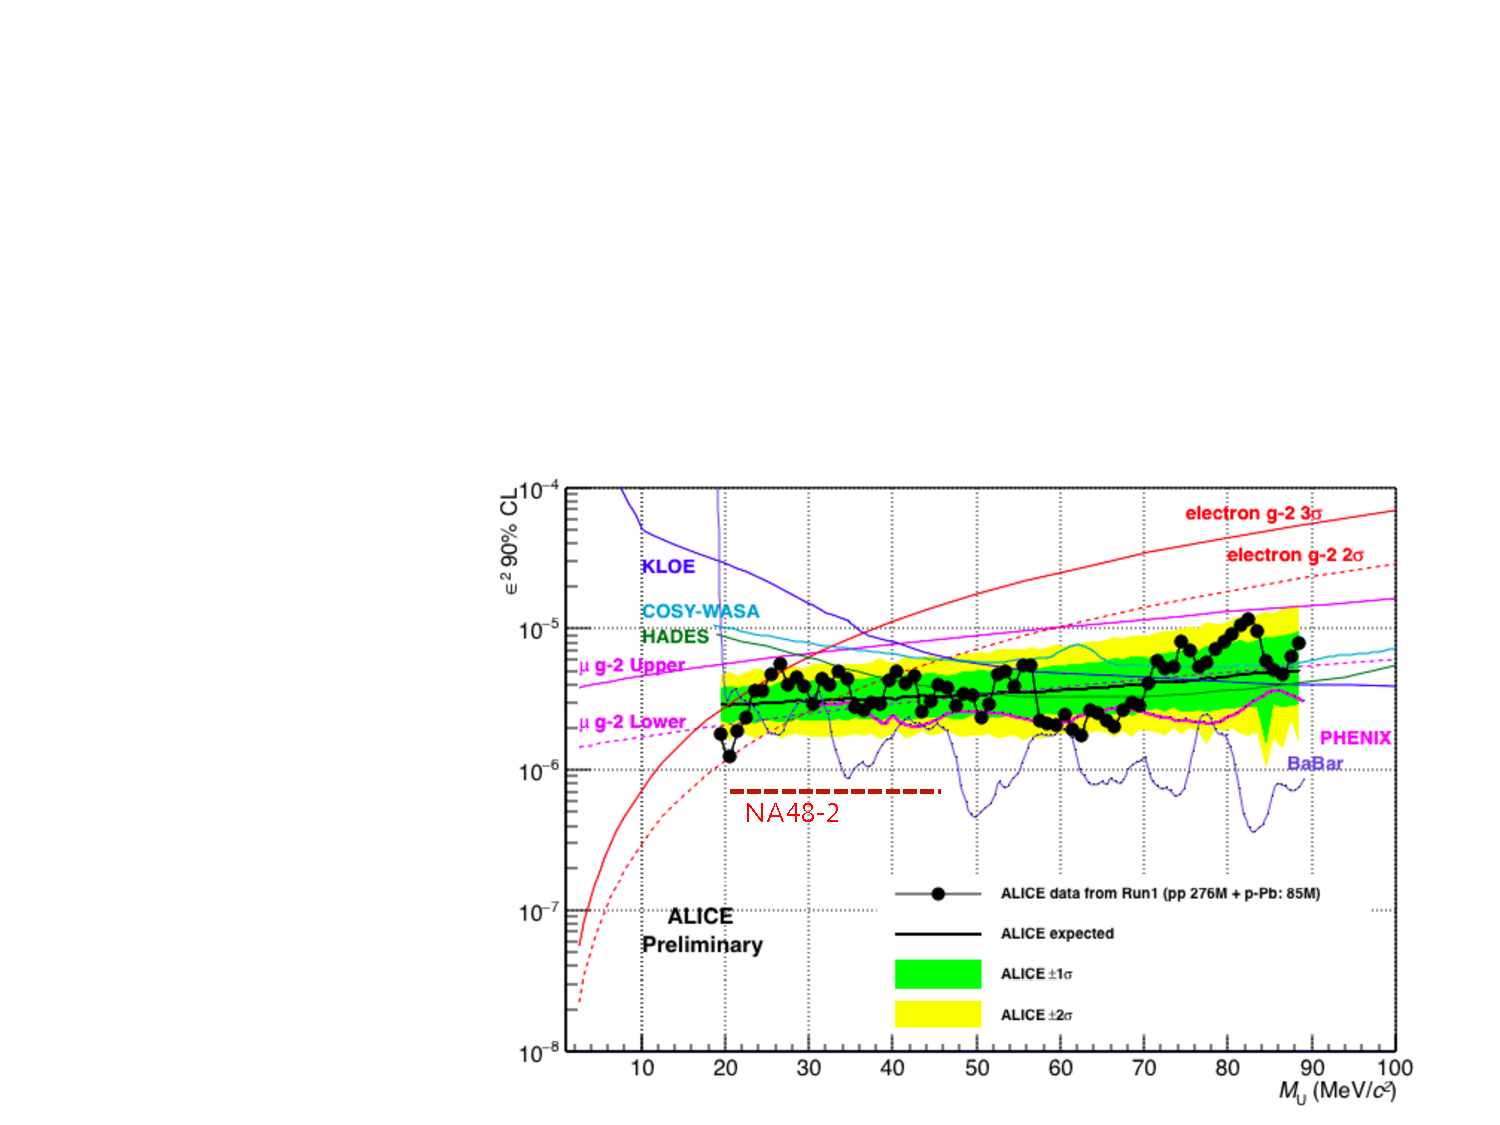
\includegraphics[width=70mm]{\main/thermalradiation/figs/darkphoton_alice_run1.pdf}
 % \end{center}
 % \caption{90\% of CL constrained by ALICE}
 % \label{fig:darkphoton_alice}
 %\end{minipage}
% \begin{minipage}{0.5\hsize}
%  \begin{center}
%   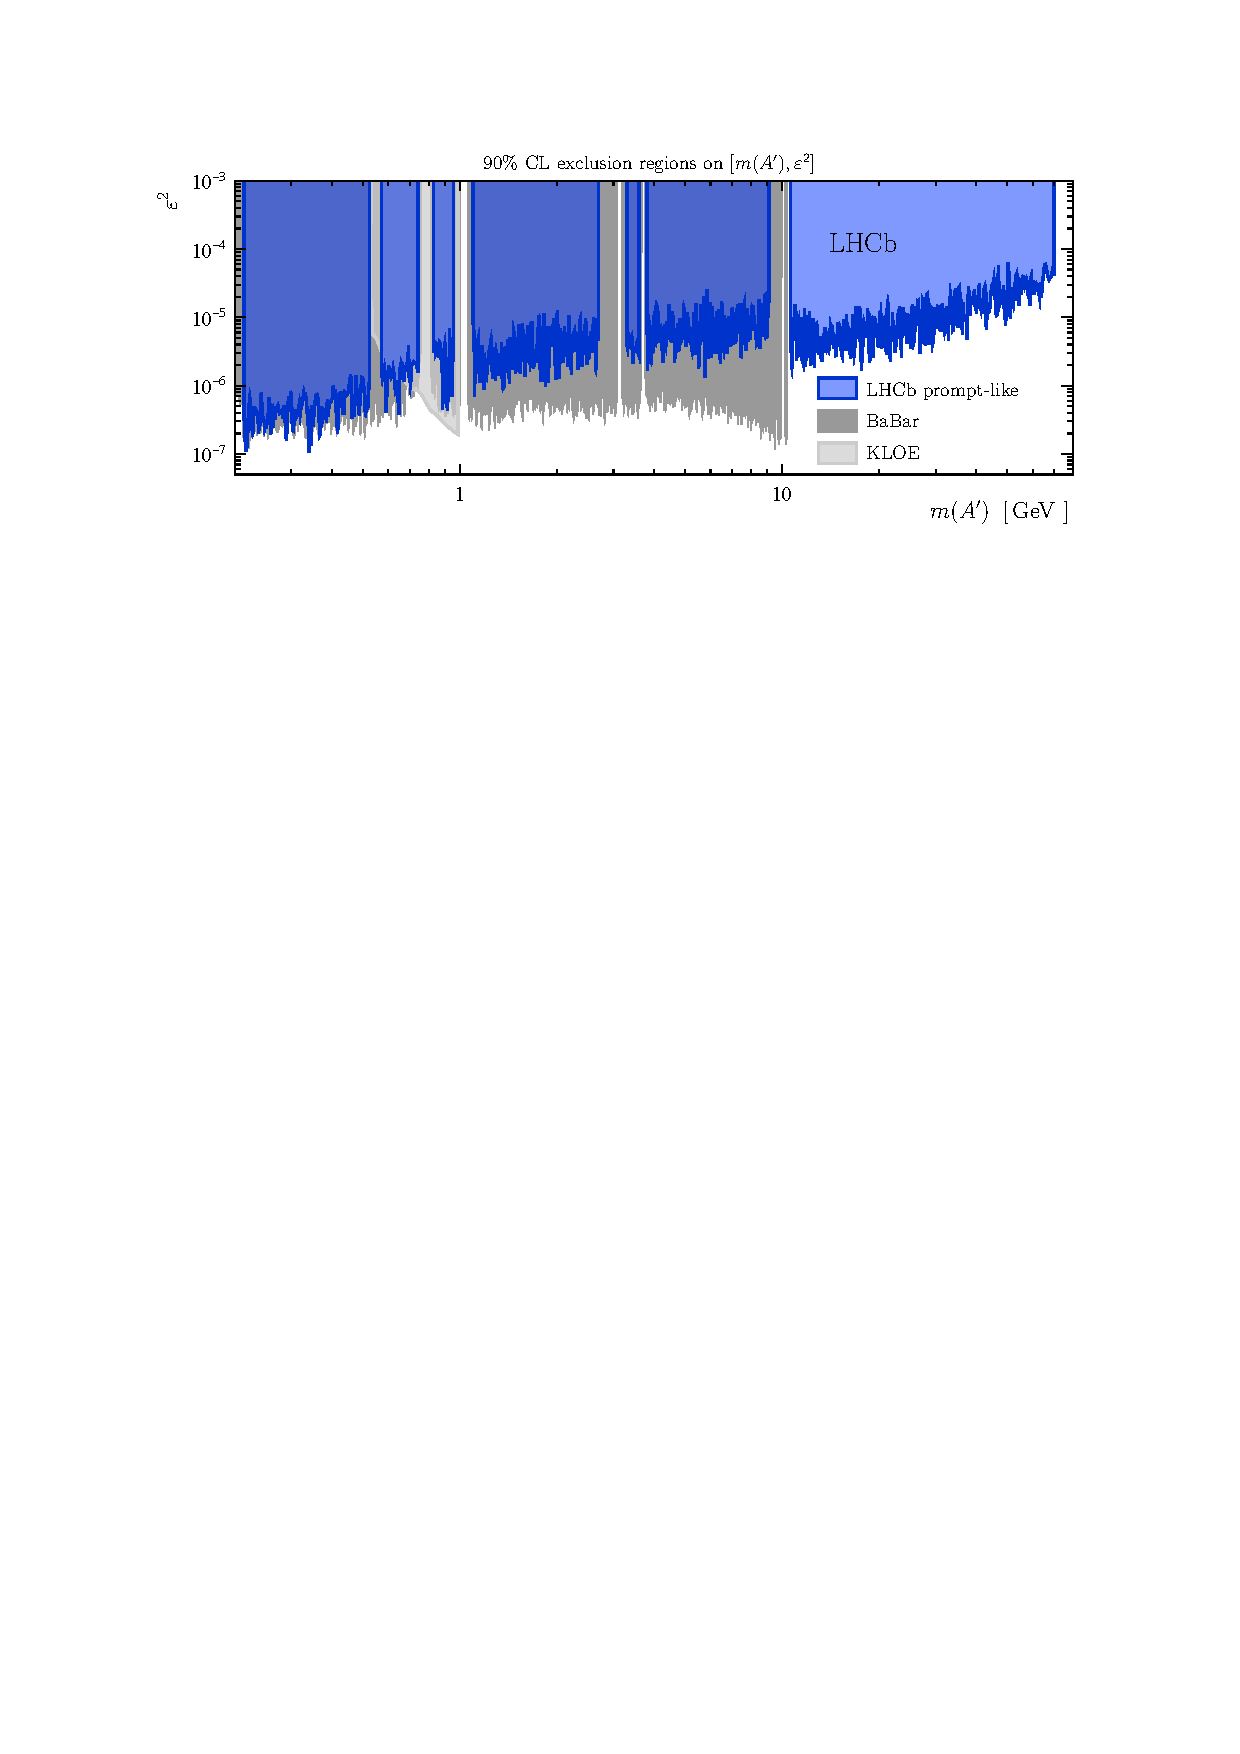
\includegraphics[width=80mm]{\main/thermalradiation/figs/darkphoton_lhcb_2016.pdf}
%  \end{center}
%  \caption{90\% of CL constrained by LHCb}
%  \label{fig:darkphoton_lhcb}
% \end{minipage}
%\end{figure}

%\subsubsection{Constraints by ALICE and LHCb from HL-LHC data}
The ALICE upgrade during LS2 will greatly improve 
the efficiency of electron-positron measurements and data taking capability.
%that enables to accumulate more collision data 
%by a factor of roughly 100 ({\bf TBC}). 
Figure~\ref{fig:darkphoton_alice_lhcb_hllhc} shows 
expected constraints that will be achieved by ALICE and LHCb
together with the future experiments. 
After the major ALICE upgrade, ALICE will accumulate 
$\unit[6]{\Upb^{-1}}$, $\unit[50]{\Unb^{-1}}$, $\unit[10]{\Unb^{-1}}$, and $\unit[3]{\Unb^{-1}}$
of \pp, \pPb, \PbPb{} collisions at \unit[0.5]{T}, and \PbPb{} collisions at \unit[0.2]{T}, 
respectively. 
%ALICE's constraint for 20 $\le m_{A'} \le $90 MeV/$c^2$ 
%will be compatible with BABAR-II experiments as shown in Fig.~\ref{fig:darkphoton_alice_lhcb_hllhc}.
LHCb will improve sensitivity of dark photon searches to large regions 
of the unexplored space. These new constraints leverage the improved invariant-mass and vertex resolution, 
as well as the unique capabilities of the particle-identification and real-time 
data-analysis with triggerless readout, 
that enables to accumulate $\Lint \sim \unit[16]{\Ufb^{-1}}$~\cite{Ilten:2016tkc}.

\begin{figure}[htbp]
\begin{center}
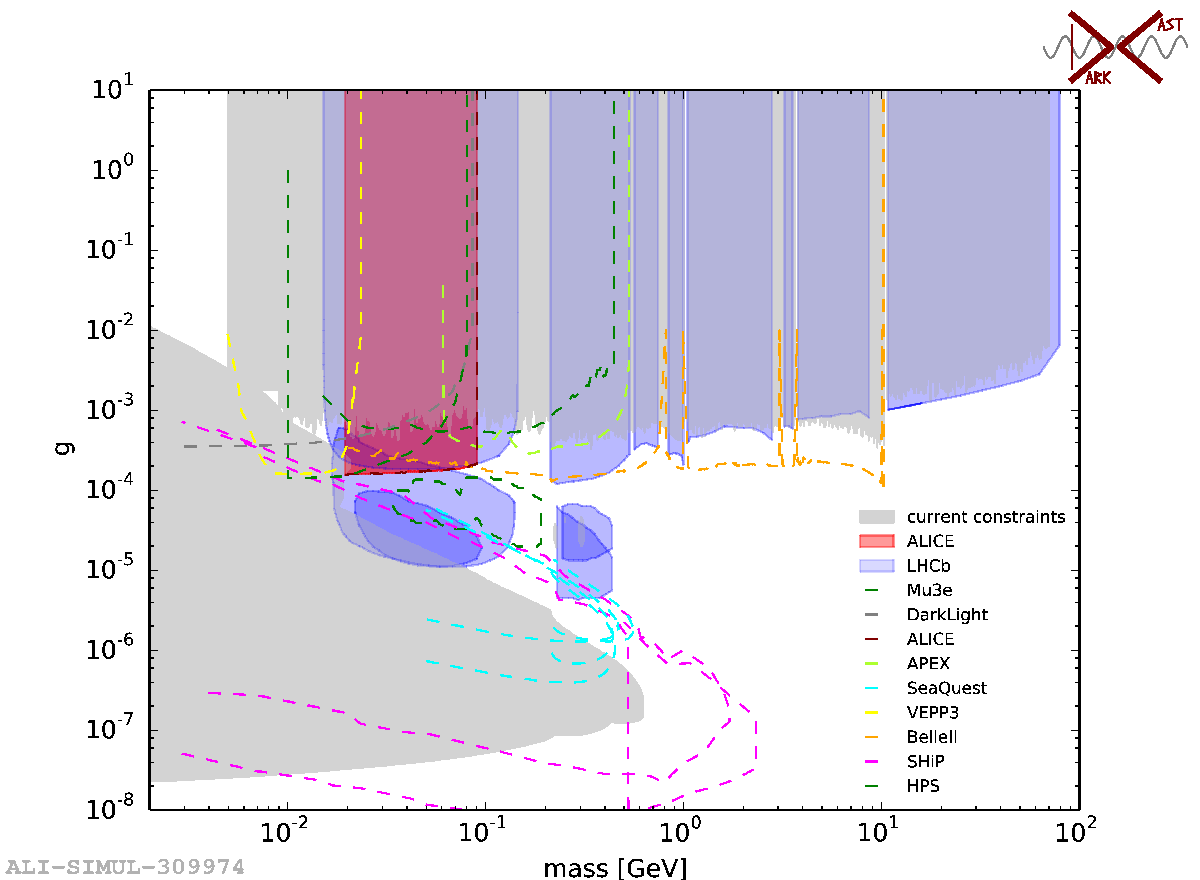
\includegraphics[width=120mm]{\main/thermalradiation/figs/2018-10-21-2018-10-21-2018-10-21-reach}
\end{center}
\caption{90\% of CL constrained by ALICE and LHCb in HL-LHC era.
Constraints by ALICE are based on 
$\unit[6]{\Upb^{-1}}$, $\unit[50]{\Unb^{-1}}$, $\unit[10]{\Unb^{-1}}$, and $\unit[3]{\Unb^{-1}}$
of \pp, \pPb, \PbPb{} collisions at \unit[0.5]{T}, and \PbPb{} collisions at \unit[0.2]{T}
and by LHC are based on $\unit[15]{\Ufb^{-1}}$.
Figures are adopted from Ref.~\cite{Ilten:2018crw}.}
\label{fig:darkphoton_alice_lhcb_hllhc}
\end{figure}

%\begin{figure}[htbp]
% \begin{minipage}{0.5\hsize}
%%  \begin{center}
 %  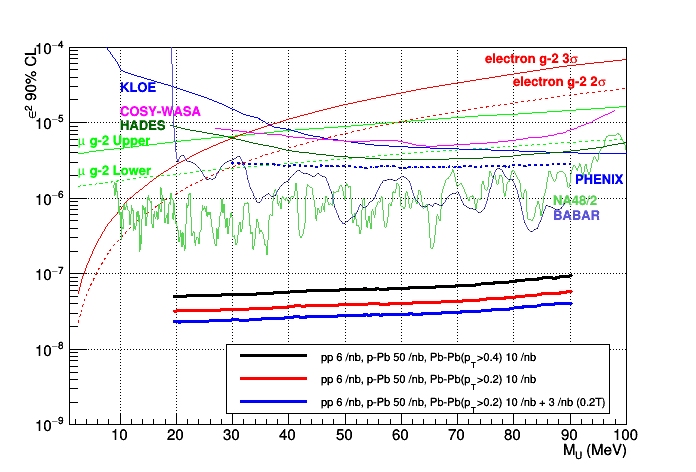
\includegraphics[width=80mm]{\main/thermalradiation/figs/dark_photon_new2_2.png}
%  \end{center}
%  \caption{90\% of CL constrained by ALICE in HL-LHC era}
%  \label{fig:darkphoton_alice_hllhc}
% \end{minipage}
% \begin{minipage}{0.5\hsize}
%  \begin{center}
%   \includegraphics[width=75mm]%%{\main/thermalradiation/figs/darkphoton_lhcb_hllhc.pdf}
%  \end{center}
%%  \caption{90\% of CL constrained by LHCb in HL-LHC era}
 % \label{fig:darkphoton_lhcb_hllhc}
 %\end{minipage}
%\end{figure}


%\begin{itemize}
%\item Preliminary Run1 results from ALICE
%\item Missing updated projections for Run 3/4 
%\item Overlap with "Dark WG"? Divide expectations in Pb-Pb and pp collisions? 
%\end{itemize}

%-----------------------------------------------------------------------%
%\begin{figure}[htb]
%\centering
%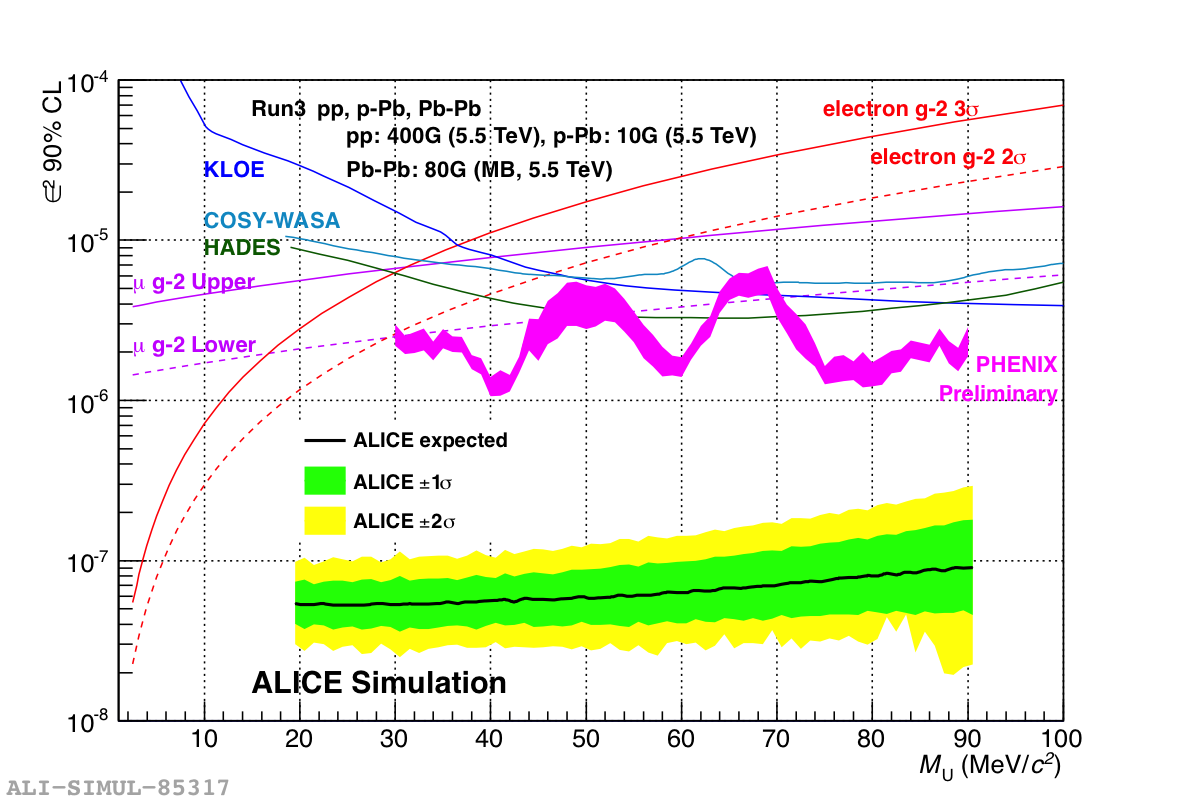
\includegraphics[width=0.85\textwidth]{\main/thermalradiation/figs/DarkPhotons}
%\caption{Placeholder: Expected performance for dark photon limits}
%\label{fig:DarkPhotons}
%\end{figure}
%-----------------------------------------------------------------------%

%\begin{itemize}
%\item Preliminary Run1 results from ALICE
%\item Missing updated projections for Run 3/4 
%\item Overlap with "Dark WG"? Divide expectations in Pb-Pb and pp collisions? 
%\end{itemize}

\subsection{Limitations and outlook}

While the statistical precision for the measurement of low mass dielectrons and dimuons as well as real photons will be sufficient in LHC Run 3 and 4 to study their yield as a function transverse momentum and with respect to the event plane (elliptic flow), more differential measurements might still be limited. 
The measurement of the photon polarization via the angular distribution of dileptons can not only provide information on the thermalization of the system, but also on the early stages of collision \cite{Baym:2017qxy}. Experimentally these distributions have been measured by the NA60 \cite{Arnaldi:2008gp}, where no polarization was found concluding that the observed excess dimuons are in agreement with the thermal emission from a a randomized system. In order to study the angular distributions, for example in the Collins-Soper reference frame \cite{Collins:1977iv,Lam:1978pu,Lam:1980uc} in the polar angle $\theta$ and the azimuthal angle $\varphi$, a large data set is needed (NA60 used $\sim50000$ excess \PGmpGmm pairs).

Another promising direction is measurement of Bose-Einstein (BE) correlations of direct photons. With this probe one can trace space-time dimensions of the hottest part of the fireball and moreover, varying \kT of the photon pair, one can select pairs coming mostly from earlier or later stages of the collision and thus look at evolution of the fireball. On the other hand, from the correlation strength parameter one can extract the direct photon spectrum down to very low $\pT \sim \unit[100]{\UMeVc}$. So far there was one successful measurement of direct photon BE correlations with WA98 collaboration \cite{Aggarwal:2003zy}, while at RHIC and LHC energies these measurements are still unavailable. The reason is that expected strength of these correlations $\lambda_{PGg}= 1/2(N_{\PGg}^{\rm dir}/N_{\PGg}^{\rm tot})^2$ is extremely small. Moreover, in contrast to massive particles, averaging of full 3D correlation function $C_2(q_{\rm out},q_{\rm side},q_{\rm long})$ to 1D $C_2(q_{\rm inv})$ results in further dramatic decrease of correlation strength \cite{Aggarwal:2003zy}. This requires very large statistics in addition to understanding the detector response. 

A first step to increase the statistical precision and the available data set for low-mass dileptons could be a further upgrade of the inner barrel of silicon detectors of the ALICE apparatus that is currently under discussion \cite{ALICE:ITS3LoI}. The planned reduction of the material budget would reduce conversion probability. In addition, an improvement of the tracking efficiency especially at low momentum would increase the conversion rejection efficiency even further. First studies \cite{ALICE:ITS3LoI} showed that the statistical uncertainty can be reduced by a factor 1.5, while the systematic uncertainty from the subtraction of the combinatorial background would be reduced by a factor 1.3. With a better pointing resolution the rejection of charm background is improved and would lead to a reduced the systematic uncertainty from the subtraction of the light-hadron and charm decay backgrounds by a factor of two. 

\end{document}
